
\chapter{Diferenciación}

Con este capítulo entramos de lleno en el terreno del Cálculo diferencial e integral.
Todo lo que hemos visto hasta ahora puede considerarse una preparación, larga y trabajosa, pero necesaria, para los temas que vamos a tratar a partir de este capítulo.

\section{Definición de derivada}

Consideremos una función $f$ definida en un intervalo abierto $(a,b)$ y sean $x_0$, $x_0+h$ puntos pertenecientes a $(a,b)$. 
La variación \emph{absoluta} de $f$ cuando $x$ se incrementa de $x_0$ a $x_0+h$ está medida por $f(x_0+h)-f(x_0)$, pero si queremos medir la variación \emph{relativa} de $f$, entonces debemos dividir esa diferencia por lo que se incrementó la variable $x$, es decir, por $h$:
\[
\text{Variación relativa de $f$ para $x$ de $x_0$ a $x_0+h$:}
\quad\frac{f(x_0+h)-f(x_0)}h.
\]
Este cociente recibe el nombre de \emph{cociente incremental}.

Ese cociente depende de $h$, pero si tomamos $h$ cada vez más pequeño, entonces tendremos una \emph{variación instantánea} de $f$ en $x_0$. Más precisamente:

\begin{definition}
Sea $f$ una función definida en un intervalo abierto $(a,b)$ y sea $x_0\in(a,b)$. Decimos que \emph{$f$ es derivable en $x_0$} si existe el límite:
\[
\lim_{h\to 0} \frac{f(x_0+h)-f(x_0)}{h}.
\]
Si este límite existe, se indica $f'(x_0)$ y se llama \emph{derivada de $f$ en $x_0$}.
\end{definition}

Es decir, \emph{la derivada de $f$ en $x_0$} es 
\[
f'(x_0) = \lim_{h\to 0} \frac{f(x_0+h)-f(x_0)}{h},
\]
siempre que el límite exista.

\begin{example}
    Consideremos la función $f(x)=x^2$. Veamos si es derivable en $x_0=2$, es decir, veamos si existe $f'(2)$:
    \begin{align*}
    f'(2) 
    &= \lim_{h\to 0}\frac{f(2+h)-f(2)}{h}
    = \lim_{h\to 0}\frac{(2+h)^2-(2)^2}{h}
    = \lim_{h\to 0}\frac{4+4h+h^2-4}{h}
    \\
    &= \lim_{h\to 0}\frac{4h+h^2}{h}
    = \lim_{h\to 0}\frac{4h}h+\frac{h^2}{h}
    = \lim_{h\to 0}4+h
    = 4+0=4.
    \end{align*}
\end{example}

La derivada de una función en un punto tiene una sencilla interpretación geométrica, en términos de la representación gráfica de dicha función. Para establecerla, consideramos la recta que pasa por los puntos de coordenadas $(x_0,y_0)=(x_0,f(x_0))$ y $(x_1,y_1)=(x_0+h,f(x_0+h))$. La pendiente de esa recta es
\[
m(h) = \frac{y_1-y_0}{x_1-x_0}
= \frac{f(x_0+h)-f(x_0)}{x_0+h-x_0}
= \frac{f(x_0+h)-f(x_0)}{h}.
\]

\centerline{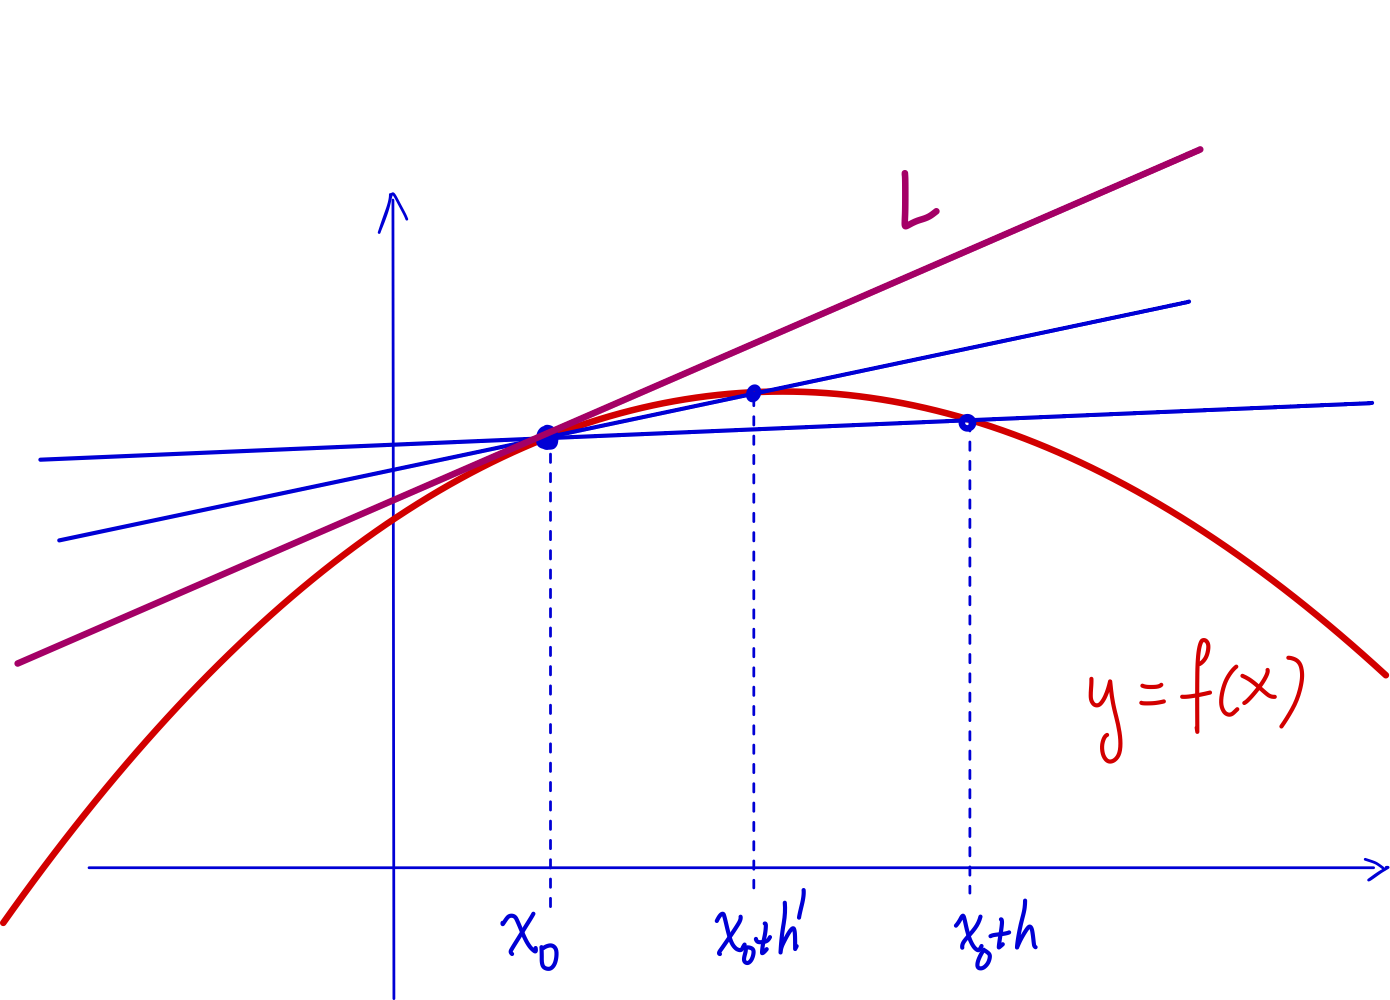
\includegraphics[width=.8\textwidth]{pics/tangente.png}}

Si ahora tomamos límite cuando $h\to 0$, vemos que la recta considerada se va aproximando a la recta $L$ tangente a la curva en el punto de coordenadas $(x_0,f(x_0))$. Por otro lado, $\lim_{h\to 0}m(h)=f'(x_0)$. Deducimos entonces lo siguiente:
\begin{quote}
    Si $f$ es una función definida en $(a,b)$ y existe $f'(x_0)$ para un $x_0\in(a,b)$, entonces $f'(x_0)$ es igual a la pendiente de la recta tangente a la gráfica de $f$ en el punto $(x_0,f(x_0))$.
\end{quote}

La ecuación de la recta tangente $L$ es ahora fácil de encontrar. Tiene pendiente $f'(x_0)$ y pasa por $(x_0,y_0)=(x_0,f(x_0))$:
\[
\frac{y-y_0}{x-x_0} = f'(x_0)
\quad\implies\quad
y - y_0 = f'(x_0)\, (x-x_0).
\]

\begin{example}
    Calculemos la ecuación de la recta tangente a la gráfica de $y=x^2$ en el punto $(x_0,y_0)=(x_0,x_0^2)$, para un $x_0\in\R$ genérico.

    Comenzamos calculando la pendiente de dicha recta, que es la derivada de $f(x)=x^2$ en $x=x_0$. Repetimos lo que hicimos en el ejemplo anterior, cambiando $2$ por $x_0$:
        \begin{align*}
    f'(x_0) 
    &= \lim_{h\to 0}\frac{f(x_0+h)-f(x_0)}{h}
    = \lim_{h\to 0}\frac{(x_0+h)^2-(x_0)^2}{h}
    = \lim_{h\to 0}\frac{x_0^2+2\, x_0\, h+h^2-x_0^2}{h}
    \\
    &= \lim_{h\to 0}\frac{2\, x_0 \, h+h^2}{h}
    = \lim_{h\to 0}\frac{2\, x_0\, \cancel{h}}{\cancel{h}}+\frac{h^{\cancel{2}}}{\cancel{h}}
    = 2\,x_0+0=2\,x_0.
    \end{align*}
    Es decir, la pendiente de la recta tangente a la gráfica de $y=x^2$ en el punto $(x_0,y_0)=(x_0,x_0^2)$ es $2 x_0$. 
    Por lo tanto, la recta tangente es la que tiene esa pendiente y  pasa por $(x_0,y_0)=(x_0,x_0^2)$:
    \[
    \frac{y-y_0}{x-x_0} = 2\, x_0
    \quad\implies\quad
    y - y_0 = 2 \, x_0\, (x-x_0)
    \quad\implies\quad
    y = x_0^2+2 \, x_0\, (x-x_0).
    \]
\end{example}

En el ejemplo anterior vimos que $f(x)=x^2$ tiene derivada en cualquier punto $x_0\in\R$ y que $f'(x_0)=2x_0$ o lo que es lo mismo, $f'(x)=2x$, para todo \xiR.



Esto no es así para todas las funciones, por ejemplo, la función \emph{valor absoluto} no es derivable en $x_0=0$.

\begin{example}
    Consideremos $f(x)=|x|$ y veamos si es derivable en $x_0=0$.
    \begin{align*}
        \lim_{h\to 0} \frac{|0+h|-|0|}h
        =
        \lim_{h\to 0} \frac{|h|}h.
    \end{align*}
    Pero 
    \[
        \lim_{h\to 0^+} \frac{|h|}h
        = \lim_{h\to 0^+} \frac{h}h = 1
        \qquad\text{y}\qquad
        \lim_{h\to 0^-} \frac{|h|}h
        = \lim_{h\to 0^-} \frac{-h}h = -1.
    \]
    Por lo tanto no existe $\lim_{h\to 0} \frac{|0+h|-|0|}h$ y $f(x)=|x|$ no es derivable en $x_0=0$.

    ?`Cuál es la recta tangente al gráfico de $y=|x|$ en el origen $(0,0)$? ?`Existe?

    Aunque sí es derivable en $x_0$ si $x_0\neq 0$.
    Queda como ejercicio verificar que
    \[
    f'(x_0) = \begin{cases}
        1,\quad&\text{si $x_0>0$},\\
        -1,\quad&\text{si $x_0<0$}.
        \end{cases}
    \]
\end{example}

La derivada tiene también una interpretación física que es importante destacar. Para establecerla, consideraremos un cuerpo desplazándose sobre una línea recta, por ejemplo, un automóvil en un tramo recto de una ruta.

Fijando una unidad de medida para las longitudes (por ejemplo, el kilómetro) y una unidad de medida para el tiempo (por ejemplo, la hora), entonces la velocidad de dicho automóvil estará medida (en kilómetros por hora) por el cociente entre el espacio que haya recorrido y el tiempo que haya empleado en recorrerlo.

Eso, desde luego, mide una velocidad promedio, pues, en el intervalo de tiempo considerado, el móvil puede haber recorrido algunas partes del trayecto más rápido que otras o, incluso, haberse detenido un rato.
Pero hay una noción de velocidad que no es un promedio, que es una noción de \emph{velocidad instantánea}, y es la que marca el velocímetro.

Independientemente de cual sea el mecanismo por el cual el velocímetro marca la velocidad en cada instante, hay una manera de llegar (teóricamente) a medir velocidades instantáneas a partir de velocidades promedio: si podemos establecer qué posición ocupa el móvil en cada instante, entonces tenemos la distancia recorrida, digamos $s$, en función del tiempo, $s=s(t)$.

Para calcular la velocidad en el instante $t_0$, comenzamos considerando un tiempo $t$ a partir de $t_0$ y calculamos la velocidad promedio entre $t_0$ y $t_0+t$:
\[
\frac{\text{distancia}}{\text{tiempo}}
=\frac{s(t_0+t)-s(t_0)}{t_0+t-t_0}
=\frac{s(t_0+t)-s(t_0)}{t}.
\]
Ahora, para calcular la velocidad en el instante $t_0$, tomamos límite en esta expresión cuando $t\to 0$. Lo que obtenemos es
\[
s'(t_0) = \lim_{t\to t_0}\frac{s(t_0+t)-s(t_0)}{t}.
\]
Deducimos entonces:
\begin{quote}
    Si, en un movimiento rectilíneo, tenemos el espacio recorrido en función del tiempo $s=s(t)$, entonces la velocidad del móvil en el instante $t_0$ está dada por la derivada de dicha función en $t_0$, es decir $s'(t_0)$.
\end{quote}

Las interpretaciones geométricas y física de la derivada tienen una notable importancia en las respectivas disciplinas, pero en este apunte sólo discutiremos (más adelante) unas pocas consecuencias geométricas, dejando el resto para los correspondientes cursos de geometría y física.

Antes de pasar a estudiar propiedades de las funciones derivables, notemos que 
\[
\lim_{h\to 0} \frac{f(x_0+h)-f(x_0)}{h}
= 
\lim_{x\to x_0} \frac{f(x)-f(x_0)}{x-x_0},
\]
que se deduce usando el cambio de variables $x=x_0+h$.

\subsection*{Definición alternativa (pero equivalente) de derivada}

Observemos que, por propiedades de límites tenemos las siguientes equivalencias:
\begin{align*}
f'(x_0) = \lim_{h\to 0} \frac{f(x_0+h)-f(x_0)}{h}
&\quad\iff\quad
f'(x_0) - \lim_{h\to 0} \frac{f(x_0+h)-f(x_0)}{h} = 0
\\
&\quad\iff\quad
\lim_{h\to 0} \bigg[f'(x_0) - \frac{f(x_0+h)-f(x_0)}{h} \bigg]= 0
\\
&\quad\iff\quad
\lim_{h\to 0} \frac{f'(x_0)\cdot h - \big(f(x_0+h)-f(x_0)\big)}{h}= 0
\\
&\quad\iff\quad
\lim_{h\to 0} \frac{f(x_0+h) - f(x_0) - f'(x_0)\cdot h}{h}= 0
\\
&\quad\iff\quad
f(x_0+h) - f(x_0) - f'(x_0)\cdot h= o(h).
\end{align*}
Es decir, $f'(x_0)$ es el número real que cumple que
\[
f(x_0+h) = f(x_0) + f'(x_0) \, h + o(h).
\]
Más precisamente
\begin{quote}
    $f$ es derivable en $x_0$ si existe un número que denotamos $f'(x_0)$ para el que se cumple que 
    \begin{equation}\label{eq:derivada-o(h)}
    f(x_0+h) = f(x_0) + f'(x_0) \, h + o(h).
    \end{equation}
\end{quote}

\begin{example}
    Veamos cómo se calcula la derivada de $f(x)=x^2$ con este método, en un $x_0\in\R$:
    \begin{align*}
        f(x_0+h) &= (x_0+h)^2 
        = \underbrace{x_0^2}_{f(x_0)} + \underbrace{2 \, x_0 }_{\text{número}} \, h + \underbrace{h^2}_{o(h)}
        = f(x_0) + \underbrace{2 \, x_0}_{f'(x_0)} \, h + o(h).
    \end{align*}
    Luego $f'(x_0)=2\, x_0$.
\end{example}

\begin{example}
    Veamos cómo se calcula la derivada de $f(x)=x^3$ con este método, en un $x_0\in\R$.
    \begin{align*}
        f(x_0+h) &= (x_0+h)^3 
        = \underbrace{x_0^3}_{f(x_0)} + \underbrace{3 \, x_0^2 }_{\text{número}} \, h + \underbrace{3 \, x_0 \, h^2+ h^3}_{o(h)}
        = f(x_0) + \underbrace{3 \, x_0^2}_{f'(x_0)} \, h + o(h).
    \end{align*}
    Luego $f'(x_0)=3\, x_0^2$.
\end{example}

\paragraph{Derivabilidad vs. Continuidad.}

La noción de derivada es \emph{puntual}, hemos definido qué quiere decir que una función es derivable \emph{en un punto $x_0$}.

Tenemos ya otra noción puntual, que es la de \emph{continuidad}. ?`Cómo se relacionan estos conceptos?

\begin{proposition}
    Si una función es derivable en $x_0$, entonces es continua en $x_0$.
\end{proposition}

\begin{proof}
    Si $f$ es derivable en $x_0$, entonces existe un número $f'(x_0)$ que cumple
    \[
    f(x_0+h) = f(x_0) + f'(x_0) \, h + o(h).
    \]
    Tomando límite cuando $h\to0$ a ambos lados tenemos que
    \begin{align*}
    \lim_{h\to 0} f(x_0+h) 
    &= \lim_{h\to 0}\big(f(x_0) + f'(x_0) \, h + o(h)\big)
    \\
    &= \lim_{h\to 0}f(x_0) \,+\, \lim_{h\to 0}f'(x_0) \, h \,+\, \lim_{h\to 0}o(h)
    \\
    &= f(x_0)+0+0=f(x_0).
    \end{align*}
    Luego, $\lim_{h\to 0}f(x_0+h)=f(x_0)$, o lo que es lo mismo,
    $\D \lim_{x\to x_0}f(x)=f(x_0)$.
\end{proof}

La recíproca de esta proposición no es cierta. Basta con pensar en la función \emph{valor absoluto}, que es continua en $x_0=0$, pero no es derivable en ese punto.

\begin{example}
    Otro ejemplo interesante es el dado por la siguiente función:
    \[
    f(x) = \begin{cases} x \sen \frac1x,\quad&\text{si $x\neq 0$},
    \\
    0, \quad&\text{si $x=0$}.
    \end{cases}
    \]
    Ya vimos en el capítulo anterior que esta función es continua en $x_0=0$ (por el teorema del emparedado).
    Veamos qué ocurre si queremos calcular $f'(0)$:
    \begin{align*}
        f'(0) 
        &= \lim_{x\to 0} \frac{f(x)-f(0)}{x-0}
        = \lim_{x\to 0} \frac{x\,\sen\frac1x - 0}{x}
        \\
        &= \lim_{x\to 0} \frac{x\,\sen\frac1x}{x}
        = \lim_{x\to 0} \sen\frac1x.
    \end{align*}
    También vimos en el capítulo anterior que este límite no existe.
    Luego, no existe $f'(0)$.
\end{example}
\subsubsection*{Ejercicios de la sección~\getcurrentref{chapter}.\getcurrentref{section}}

\begin{enumerate}
\item Calcular las siguientes derivadas usando la definición:
\begin{multicols}{2}
    \begin{enumerate}
        \item $f'(1)$ para $f(x)=2x+3$
        \item $f'(2)$ para $f(x)=3x^2-1$
        \item $f'(4)$ para $f(x)=\sqrt{x}$
        \item $f'(2)$ para $f(x)=1/x$
    \end{enumerate}
\end{multicols}
\item Determinar si la siguiente función es derivable en $x_0=0$:
\[
    f(x) = \begin{cases} x^2 \sen \frac1x,\quad&\text{si $x\neq 0$},
    \\
    0, \quad&\text{si $x=0$}.
\end{cases}
\]
\item Hallar usando la definición, la derivada de $f:(0,+\infty)\to R$ dada por $f(x)=\sqrt{x}$.
Plantear el cociente incremental y multiplicar por \emph{el conjugado}.
\end{enumerate}


\section{La función derivada. Reglas de derivación}

Supongamos que $f$ está definida en un intervalo abierto $(a,b)$ y que es derivable en todos los puntos de $(a,b)$.
Cuando esto ocurre, diremos que \emph{$f$ es derivable en $(a,b)$}.
Para cada $x\in(a,b)$ tenemos una derivada $f'(x)$. De esta manera, tenemos definida una función:
\[
x \to f'(x),
\]
que se llamará \emph{función derivada de $f$} y se indica $f'$.

%\subsection{Reglas de derivación}

Para seguir adelante con el cálculo de derivadas. Necesitamos tres propiedades que nos indican cómo se comporta la derivada frente a las operaciones elementales de funciones: la suma el producto y el cociente.

\begin{proposition}
    Si $f$ es derivable en $x_0$ y $c$ es una constante, entonces $c\, f$ es derivable en $x_0$ y además
    \[
    (c\, f)'(x_0) = c \, f'(x_0).
    \]
    En palabras: \emph{la derivada de una constante por una función es la constante por la derivada de la función}.
\end{proposition}

\begin{proof}
Utilizaremos la definición alternativa dada en~\eqref{eq:derivada-o(h)}.
Llamamos $g(x)=c\, f(x)$ y por la propiedad distributiva, obtenemos
\begin{align*}
    g(x_0+h) &= (c \, f)(x_0+h) = c \, f(x_0+h) 
    \\
    &= c\, \big( f(x_0) + f'(x_0)\cdot h + o(h) \big) 
    \\
    &=  c\, f(x_0) + c\, f'(x_0)\cdot h + c\, o(h)
    \\
    &=  g(x_0) + c\, f'(x_0)\cdot h +  o(h).
\end{align*}    
Por lo tanto $g'(x_0) = c\, f'(x_0)$.
\end{proof}

\begin{example}
    Ya sabemos que la derivada de $x^2$ es $2\, x$, por lo tanto, 
    \[
    \text{la derivada de $5 x^2$ es  $5 \cdot 2 \, x = 10\,  x$.}
    \]
\end{example}

\begin{proposition}
    Si $f$ y $g$ son derivables en $x_0$, entonces $f+g$ es derivable en $x_0$ y además
    \[
    (f+g)'(x_0) = f'(x_0)+g'(x_0).
    \]
    En palabras: \emph{la derivada de la suma es la suma de las derivadas}.
\end{proposition}

\begin{proof}
Utilizaremos la definición alternativa dada en~\eqref{eq:derivada-o(h)}.
\begin{align*}
    (f+g)(x_0+h) 
    &= f(x_0+h)+g(x_0+h)
    \\
    &= \big[f(x_0)+f'(x_0)\, h + o(h)\big]
    + \big[g(x_0)+g'(x_0)\, h + o(h)\big]
    \\
    &= \big[f(x_0)+g(x_0)\big] +
    \big[f'(x_0)\, h + g'(x_0)\, h\big] 
    + \big[o(h)+ o(h)\big]
    \\
    &= (f+g)(x_0) +
    \big[f'(x_0)+ g'(x_0)\big] \, h
    + o(h).
\end{align*}
Por lo tanto $(f+g)'(x_0) = f'(x_0)+g'(x_0)$.
\end{proof}

\begin{example}
    Ya sabemos que la derivada de $5 \,x^2$ es $10\,x$, y que la de $x^3 = 3\, x^2$.
    Por lo tanto, 
    \[
    \text{la derivada de $5 x^2 + 6 x^3$ es $10 \, x + 6 \cdot 3 \, x^2 = 10 x + 18 x^2$.}
    \]
\end{example}

\begin{proposition}
    Si $f$ y $g$ son derivables en $x_0$, entonces $f\cdot g$ es derivable en $x_0$ y además
    \[
    (f\cdot g)'(x_0) = f'(x_0)\cdot g(x_0)+f(x_0)\cdot g'(x_0).
    \]
\end{proposition}

\begin{proof}
Utilizaremos la definición alternativa dada en~\eqref{eq:derivada-o(h)}.
Por la propiedad distributiva,
\begin{align*}
    (f\cdot g)(x_0+h) 
    ={}& f(x_0+h)\cdot g(x_0+h)
    \\
    ={}& \big[f(x_0)+f'(x_0)\, h + o(h)\big]
    \cdot \big[g(x_0)+g'(x_0)\, h + o(h)\big]
    \\
    ={}& f(x_0)\cdot g(x_0) 
    + f'(x_0)\cdot g(x_0) 
    + \underbrace{o(h) \cdot g(x_0) }_{o(h)}
    \\
    &+ f(x_0) \cdot g'(x_0) \, h
    + \underbrace{f'(x_0) \, h \cdot g'(x_0) \, h}_{o(h)}
    + \underbrace{o(h) \cdot g'(x_0) \, h}_{o(h)}
    \\
    &
    + \underbrace{f(x_0) \cdot o(h)}_{o(h)}
    + \underbrace{f'(x_0) \cdot o(h)}_{o(h)}
    + \underbrace{o(h) \cdot o(h)}_{o(h)}
    \\
    ={}& f(x_0)\cdot g(x_0) 
    + \big[ f'(x_0)\cdot g(x_0)+f(x_0)\cdot g'(x_0) \big] \, h 
    + o(h).
\end{align*}
Por lo tanto $(f\cdot g)'(x_0) = f'(x_0)\cdot g(x_0)+f(x_0)\cdot g'(x_0)$.
\end{proof}

\begin{proposition}
    Si $g$ es derivable en $x_0$, y $g(x_0)\neq 0$, entonces $1/g$ es derivable en $x_0$ y además
    \[
    \Big(\frac1g\Big)'(x_0) = - \frac{g'(x_0)}{g(x_0)^2}.
    \]
\end{proposition}

\begin{proof}
    Analicemos el cociente incremental:
    \begin{align*}
         % \frac{\frac1g(x_0+h)-\frac1g(x_0)}h
        \frac{\frac1{g(x_0+h)}-\frac1{g(x_0)}}h
        &= \frac1h \, \left[\frac1{g(x_0+h)}-\frac1{g(x_0)}\right]
        = \frac1h \, \frac{g(x_0)-g(x_0+h)}{g(x_0+h)\,g(x_0)}
        \\
        &= \frac1{g(x_0+h)\,g(x_0)} \, \frac{g(x_0)-g(x_0+h)}h
        \\
        &= - \frac1{g(x_0+h)\,g(x_0)} \, \frac{g(x_0+h)-g(x_0)}h.
    \end{align*}
    Recordamos ahora que como $g$ es derivable en $x_0$ es también continua, y por hipótesis, $g(x_0)\neq 0$. 
    Luego, 
    \[
    \limho \frac1{g(x_0+h)\,g(x_0)} = \frac1{g(x_0)\,g(x_0)} = \frac1{g(x_0)^2}. 
    \]
    Además, $\limho \frac{g(x_0+h)-g(x_0)}h = g'(x_0)$.
    Finalmente,
    \[
    \left(\frac1g\right)'(x_0) = \limho \frac{\frac1{g(x_0+h)}-\frac1{g(x_0)}}h = - \frac{g'(x_0)}{g(x_0)^2}.
    \qedhere
    \]
\end{proof}

Combinando este último resultado con la regla para el producto, obtenemos la regla de derivación para el cociente:

\begin{corollary}
    Si $f$ y $g$ son derivables en $x_0$, y $g(x_0)\neq 0$, entonces $f/ g$ es derivable en $x_0$ y además
    \[
    \left(\frac f g\right)'(x_0) = \frac{f'(x_0)\cdot g(x_0)-f(x_0)\cdot g'(x_0)}{g(x_0)^2}.
    \]
\end{corollary}

\begin{proof}
Como $\D\frac fg = f \cdot \frac1g$ tenemos que
    \begin{align*}
        \left(\frac f g\right)'(x_0) 
        &= \left(f \cdot \frac 1 g\right)'(x_0)
        = f'(x_0) \left(\frac 1 g\right)(x_0) + f(x_0) \left(\frac 1 g\right)'(x_0).
    \end{align*}
Como $g$ es derivable en $x_0$ y $g(x_0)\neq 0$, tenemos que $\left(\frac1g\right)'(x_0) = - \frac{g'(x_0)}{g(x_0)^2}$ y entonces
    \begin{align*}
        \left(\frac f g\right)'(x_0) 
        &= f'(x_0) \frac 1 {g(x_0)} + f(x_0) \left(- \frac{g'(x_0)}{g(x_0)^2}\right)
        = \frac{f'(x_0)\cdot g(x_0)-f(x_0)\cdot g'(x_0)}{g(x_0)^2}.
        \qedhere
    \end{align*}
\end{proof}

Podemos resumir los últimos resultados de la siguiente manera:
\[
(c\, f)' = c\, f',
\qquad
(f+g)' = f'+g',
\qquad
(f\cdot g)' = f'g+f g',
\qquad
\left(\frac f g\right)' = \frac{f'g-f g'}{g^2},
\]
donde la última fórmula tiene sentido en los puntos $x$ donde $g(x)\neq 0$.
Es importante observar que si bien la derivada de la suma es la suma de las derivadas, no es cierto que la derivada del producto es el producto de las derivadas, ni que la derivada del cociente es el cociente de las derivadas.

\paragraph{Notación de Leibniz.}
Otra manera muy usual de denotar a las derivadas es la siguiente, conocida como notación de Leibniz:
\[
f'(x)= \frac{df(x)}{dx}, \qquad\text{o también}\quad f'= \frac{df}{dx}.
\]
Si estamos pensando que $y=f(x)$, es decir, $y$ es la variable \emph{dependiente}, definida como $f(x)$, entonces también suele escribirse
\[
f'(x) = \frac{dy}{dx}.
\]
Esta forma es muy útil cuando uno quiere representar la derivada de una función \emph{anónima}, es decir una función que no tiene nombre asignado. Por ejemplo:
\[
\frac{d (x^2)}{dx} = 2x,
\qquad
\frac{d (5 \, x^2)}{dx} = 5 \frac{d (x^2)}{dx} =5\cdot 2x = 10x.
\]

Con la notación de Leibniz, las reglas de derivación recién presentadas pueden escribirse de la siguiente forma:
\[
\frac{d(c\, f)}{dx} = c\, \frac{df}{dx},
\quad
\frac{d(f+g) }{dx} = \frac{d f}{dx}+\frac{d g}{dx},
\quad
\frac{d(f\cdot g)}{dx} = \frac{df}{dx}g+f \frac{dg}{dx},
\quad
\frac{d\big(\frac f g\big)}{dx} = \frac{\frac{df}{dx}g-f \frac{dg}{dx}}{g^2}.
\]

Finalizamos esta sección aprovechando la regla del producto para saber cuál es la derivada de $f(x) = x^n$ para $n\in\N$.
El caso $n=1$ nos da $f(x)=x$ y $f'(x)=1$, es decir $\frac{dx}{dx}=1$. El caso $n=2$ nos da $\frac{d(x^2)}{dx}=2x$, el caso $n=3$ nos da $\frac{d(x^3)}{dx}=3x^2$. En el caso general, para $n\in\N$, la derivada de $x^n$ será $$\frac{d(x^n)}{dx}=n x^{n-1}$$ y lo vamos a probar por inducción. Ya hemos probado el caso $n=1$ (y también los casos $n=2$ y $n=3$). Supongamos que esta fórmula es válida para un cierto natural $n$ y veamos si es cierta para $n+1$. Observamos que $x^{n+1} = x^n \cdot x$, y utilizando la regla del producto:
\[
\frac{d(x^{n+1})}{dx}
=
\frac{d(x^n\cdot x)}{dx}
= 
\frac{d(x^n)}{dx} x + x^n \frac{dx}{dx}.
\]
Por la hipótesis inductiva, $\frac{d(x^n)}{dx}=n\, x^{n-1}$, así que
\[
\frac{d(x^{n+1})}{dx}
= n\, x^{n-1} \, x + x^n \cdot 1
= n x^n + x^n = (n+1)x^n.
\]

Por lo tanto, todas las funciones polinomiales son derivables, y más aún, 
\begin{multline*}
\text{Si }p(x) = a_n \, x^n + a_{n-1} \, x^{n-1} + \dots + a_2 \, x^2 + a_1 \, x + a_0
\\
\quad\text{\ \ entonces \ \ }
p'(x) = n\, a_n \, x^{n-1} + (n-1) \, a_{n-1} \, x^{n-2} + \dots + 2\, a_2 \, x + a_1.
\end{multline*}

Y por la regla del cociente, también todas las funciones racionales son derivables en todo punto de su dominio (todos los puntos donde el denominador no se anula).


\subsection*{Derivadas de orden superior.}
Como vimos al principio de esta sección, si una función $f$ es derivable, podemos formar una nueva función $f'$, la derivada de $f$. Si $f'$ es a su vez derivable, podemos tomar su derivada $(f')'$, llamada \emph{derivada segunda de $f$} y se designa por $f''$. Si esta función es derivable, podemos volver a calcular su derivada, que será la derivada tercera y se denotará $f'''$, etc. Para derivadas de orden superior a $3$, denotaremos el orden de las derivadas con un supra-índice entre paréntesis. Por ejemplo, la derivada cuarta es $f^{(4)}$, y la $n$-ésima es $f^{(n)}$.
Por ejemplo, si $f(x)=x^5$, tenemos que
\[
f'(x)=5\,x^4,\quad
f''(x)=20\,x^3,\quad
f'''(x)=60\,x^2,\quad
f^{(4)}(x)=120\,x,\quad
f^{(5)}(x)=120,
\]
y $f^{(6)}(x)=0$, con $f^{(n)}(x)=0$, para todo $n\ge 6$.

También podemos usar la notación de Leibniz para las derivadas de orden superior. Si $y=x^5$,
\[
\dd{y}{x}=5\,x^4,\quad
\dd[2]{y}{x}=20\,x^3,\quad
\dd[3]{y}{x}=60\,x^2,\quad
\dd[4]{y}{x}=120\,x,\quad
\dd[5]{y}{x}=120,\quad
\]
con $\D\dd[n]{f}{x}=0$, para todo $n\ge 6$.




\subsubsection*{Ejercicios de la sección~\getcurrentref{chapter}.\getcurrentref{section}}

\begin{enumerate}
\item Hallar $f'(x)$ siendo $f(x)$ igual a:
\begin{multicols}{2}
\begin{enumerate}
    \item $\D 3x^3+6x^2-2x+1$
    \item $\D x(3+x^2)$
    \item $\D 4x(2+x^3+5x^4)$
    \item $\D (x+2)(x+3)(3x+1)(2+5x^2)$
    \item $\D \frac{x-1}x$
    \item $\D \frac{4x-3}{2x+4}$
    \item $\D \frac{(x+3)^2(4x-1)}{(2x+1)^2(3x-2)}$
    \item $\D \frac{x^3}{(4-x^2)^2}$
    \item $\D 4x-\frac2x$
\end{enumerate}
\end{multicols}

\item Calcular las siguientes derivadas:
\begin{multicols}{2}
\begin{enumerate}
    \item $\D \dd[3]{}{x} \big(3x^3+6x^2-2x+1\big)$
    \item $\D \dd[4]{}{x}\big(x(3+x^2)\big)$
    \item $\D \dd[2]{}{x}\big((x+2)(x+3)(3x+1)(2+5x^2)\big)$
    \item $\D \dd[2]{}{x}\frac{x-1}x$
\end{enumerate}
\end{multicols}

\item Sea $f(x)=x^n$, para \niN. Hallar $f^{(k)}(x)$, para
\begin{multicols}{3}
    \begin{enumerate}
    \item $k=n$;
    \item $k>n$;
    \item $k<n$.
\end{enumerate}
\end{multicols}

\item Dada la función polinómica $\D p(x)=a_n x^n + a_{n-1} x^{n-1} + \dots + a_1 x + a_0$:
\begin{multicols}{2}
    \begin{enumerate}
    \item Hallar $\D \dd[n]{p(x)}{x}$;
    \item Hallar $\D \dd[k]{p(x)}{x}$, para $k>n$.
\end{enumerate}
\end{multicols}


\end{enumerate}


\section{Ejemplos importantes}

La potencia del Cálculo Diferencial en sus diversas aplicaciones depende del hecho siguiente: es muy fácil probar que casi todas las funciones hasta aquí estudiadas (polinómicas, trigonométricas, logarítmicas, etc.) son derivables en todo su dominio, y es muy fácil encontrar sus funciones derivadas. Veamos cómo.

\begin{example}
    Consideremos la función constante $f(x)=c$, para todo \xiR. Su derivada es la función nula. En efecto, para \xiR,
    \[
    \frac{f(x+h)-f(x)}{h} = \frac{c-c}h = \frac0h = 0,\ \ \forall h\neq 0
    \quad\implies\quad
    \lim_{h\to0}\frac{f(x+h)-f(x)}{h} = 0.
    \]
\end{example}

\begin{example}
    La derivada de la función identidad $f(x)=x$ es también fácil de encontrar.  En efecto, para \xiR,
    \[
    \frac{f(x+h)-f(x)}{h} = \frac{x+h-x}h = \frac hh = 1,\ \ \forall h\neq 0
    \quad\implies\quad
    \lim_{h\to0}\frac{f(x+h)-f(x)}{h} = 1.
    \]
    Luego, para la función identidad $f(x)=x$, resulta $f'(x)=1$.
\end{example}

\begin{example}
    Ya vimos que la derivada de $f(x)=x^2$ es $f'(x)=2x$, y que la derivada de $g(x)=x^3$ es $g'(x)=3x^2$.
\end{example}

\begin{example}
    Consideremos ahora un ejemplo un poquito más complicado, que es el de la función \emph{seno}.
    Utilizaremos ahora la identidad trigonométrica que dice que
    \[
    \sen(a)-\sen(b) = 2 \cos\big(\frac{a+b}2\big) \sen\big(\frac{a-b}2\big), 
    \quad\text{para todo $a,b\in\R$}.
    \]
    Sea $f(x)=\sen(x)$. Planteamos el cociente incremental 
    \begin{align*}
        \lim_{h\to0} \frac{f(x+h)-f(x)}{h} 
        &= 
        \lim_{h\to0} \frac{\sen(x+h)-\sen(x)}{h} 
        = 
        \lim_{h\to0} \frac{2\cos\big(\frac{x+h+x}2\big)\sen\big(\frac{x+h-x}2\big)}{h} 
        \\
        &= 
        \lim_{h\to0} \cos\big(\frac{2x+h}2\big)\frac{2\sen\big(\frac{h}2\big)}{h} 
        = 
        \lim_{h\to0} \cos\big(x+\frac{h}2\big)\frac{\sen\big(\frac{h}2\big)}{h/2} 
        \\
        &= 
        \lim_{h\to0} \cos\big(x+\frac{h}2\big) \lim_{h\to0}  \frac{\sen\big(\frac{h}2\big)}{h/2} 
        = \cos(x) \cdot 1 = \cos (x),
    \end{align*}
    donde hemos utilizado que la función coseno es continua (que implica $\lim_{h\to 0}\cos(x+\frac h2)=\cos(x)$), y que $\lim_{y\to0}\sen(y)/y=1$.
    Por lo tanto, la derivada de la función $f(x)=\sen(x)$ es $f'(x)=\cos(x)$.
\end{example}

\begin{example}
    Veamos ahora cuál es la derivada de la función \emph{coseno}.
    Utilizaremos ahora la identidad trigonométrica que dice que
    \[
    \cos(a)-\cos(b) = -2 \sen\big(\frac{a+b}2\big) \sen\big(\frac{a-b}2\big), 
    \quad\text{para todo $a,b\in\R$}.
    \]
    Sea $f(x)=\cos(x)$. Planteamos el cociente incremental:
    \begin{align*}
        \lim_{h\to0} \frac{f(x+h)-f(x)}{h} 
        &= 
        \lim_{h\to0} \frac{\cos(x+h)-\cos(x)}{h} 
        =
        \lim_{h\to0} \frac{-2 \sen\big(\frac{x+h+x}2\big) \sen\big(\frac{x+h-x}2\big)}h
        \\
        &= 
        \lim_{h\to0} -\sen\big(x+\frac h2\big) \frac{\sen\big(\frac h2\big)}{h/2}
        = 
        -\lim_{h\to0} \sen\big(x+\frac h2\big) \lim_{h\to0} \frac{\sen\big(\frac h2\big)}{h/2}
        \\
        &= -\sen(x) \cdot 1 = -\sen(x),
    \end{align*}
    donde hemos utilizado que la función seno es continua (que implica $\lim_{h\to 0}\sen(x+\frac h2)=\sen(x)$), y nuevamente que $\D\lim_{y\to0}\sen(y)/y=1$.
    Por lo tanto, la derivada de la función $f(x)=\cos(x)$ es $f'(x)=\sen(x)$.
\end{example}

\begin{example}
    Consideremos ahora la función logaritmo natural $f(x)=\ln x$, con dominio $(0,+\infty)$. Planteamos el cociente incremental:
    \begin{align*}
        \frac{f(x+h)-f(x)}{h} 
        &= 
        \frac{\ln(x+h)-\ln(x)}h
        =
        \frac{\ln\big(\frac{x+h}x\big)}h
        =
        \frac1h \ln\big(\frac{x+h}x\big)
        \\
        &= 
        \ln \big(\frac{x+h}x\big)^{1/h}
        = \ln \big(1+\frac{h}{x}\big)^{1/h}
        = \ln \big(1+\frac{1}{x/h}\big)^{1/h}
        \\
        &= \ln\bigg( \big(1+\frac{1}{x/h}\big)^{x/h} \bigg)^{1/x}
        = \frac1x \ln \big(1+\frac{1}{x/h}\big)^{x/h}.
    \end{align*}        
    Ahora bien, con el cambio de variables $y=\frac xh$, como $\lim_{h\to 0}y = \infty$,
    \[
    \lim_{h\to 0} \big(1+\frac{1}{x/h}\big)^{x/h} 
    = \lim_{y\to\infty} \big(1+\frac{1}{y}\big)^{y}
    = e.
    \]
    Por lo tanto, $\lim_{h\to 0} \ln \big(1+\frac{1}{x/h}\big)^{x/h} =\ln e = 1$ y finalmente
    \[
    \lim_{h\to0}  \frac{\ln(x+h)-\ln(x)}h
        = \frac1x \cdot 1 = \frac1x.
    \]
    Es decir, la derivada de la función logaritmo natural $f(x)=\ln x$ es $\D f'(x)=\frac1x$.
\end{example}

\begin{example}
    Por último, estudiemos la derivada de la función exponencial $f(x)=e^x$.
     Planteamos el cociente incremental:
    \begin{align*}
        \frac{f(x+h)-f(x)}{h} 
        &= \frac{e^{x+h}-e^x}h
        = \frac{e^x \, e^h-e^x}h
        = \frac{e^x \big(e^h-1\big)}h
        = e^x \frac{e^h-1}h.
    \end{align*}
    Tenemos entonces que calcular $\limho \frac{e^h-1}h$. Hacemos el cambio de variable $y=e^h-1$ y observamos, por un lado, que $$\limho\, y = \limho (e^h-1) = e^0-1=1-1=0.$$
    Por otro lado, si $y=e^h-1$, entonces $e^h=1+y$ y $h=\ln(1+y)$. Luego,
    \begin{align*}
        \limho \frac{e^h-1}h 
        = \lim_{y\to0} \frac{y}{\ln(1+y)}
        = \lim_{y\to0} \frac{1}{\frac1y\ln(1+y)}
        = \lim_{y\to0} \frac{1}{\ln(1+y)^{1/y}}.
    \end{align*}
    Como vimos recién, $\lim_{y\to 0} (1+y)^{1/y}=e$, por lo que 
    $\lim_{y\to 0} \ln (1+y)^{1/y}=\ln e=1$, y finalmente
    \[
    \limho  \frac{e^{x+h}-e^x}h
    = e^x \limho \frac{e^h-1}h 
    = e^x \lim_{y\to0} \frac{1}{\ln(1+y)^{1/y}}
    = e^x \cdot 1 = 1.
    \]
    Es decir, la derivada de la función exponencial $f(x)=e^x$ es $f'(x)=e^x$.
\end{example}

Podemos resumir los resultados anteriores de la siguiente manera:

\noindent\hfil
\begin{minipage}{.4\textwidth}
\def\arraystretch{1.8}
\begin{tabular}{|c|c|}
    \hline
    $f(x)$ & $f'(x)$ \\
    \hline\hline
    $\D c$ (constante) 
    & $\D 0$
    \\ \hline
    $\D x^n$ 
    & $\D nx^{n-1}$
    \\ \hline
    $\D \sen x$ 
    & $\D \cos x$
    \\ \hline
    $\D \cos x$ 
    & $\D -\sen x$
    \\ \hline
    $\D \ln x$ 
    & $\D \frac1x$
    \\ \hline
    $\D e^x$ 
    & $\D e^x$
    \\ \hline
\end{tabular}
\end{minipage}
\hfil
\begin{minipage}{.4\textwidth}
\begin{align*}
    \frac{dc}{dx} &= 0 \\[5pt]
    \frac{d(x^n)}{dx} &= n x^{n-1}\\[5pt]
    \frac{d\sen x }{dx } &= \cos x  \\[5pt]
    \frac{d \cos x}{dx } &= -\sen x  \\[5pt]
    \frac{d\ln x }{dx } &=  \frac1x \\[5pt]
    \frac{d e^x}{dx } &= e^x
\end{align*}
\end{minipage}

Es importante notar que el procedimiento que nos llevó a las fórmulas de la tabla precedente, por un lado demuestra que todas las funciones consideradas son derivables en todo punto de su dominio, y por otro lado nos dice explícitamente cuánto valen sus derivadas en cualquier punto.

\subsubsection*{Ejercicios de la sección~\getcurrentref{chapter}.\getcurrentref{section}}

\begin{enumerate}
\item Hallar $f'(x)$ siendo $f(x)$ igual a:
\begin{multicols}{2}
\begin{enumerate}
    \item $\D \tan x$
    \item $\D \cotan x$
    \item $\D \sec x$
    \item $\D \cosec x$
    \item $\D \frac{x+e^x}{5-x^2}+\tan x$
    \item $\D x \ln x$
\end{enumerate}
\end{multicols}

\item Se definen las funciones hiperbólicas de la siguiente manera:
\[
\cosh x = \frac{e^x+e^{-x}}{2},
\qquad
\senh x = \frac{e^x-e^{-x}}{2}
\]
\begin{enumerate}
    \item Probar que $\cosh^2 x-\senh^2 x = 1$
    \item Probar que $\D\dd{\senh x}{x} = \cosh x$
    \item Probar que $\D\dd{\cosh x}{x} = \senh x$
\end{enumerate}

\item Hallar una fórmula para la derivada de $\log_a x$.

\item Hallar las siguientes derivadas:
\begin{multicols}{2}
    \begin{enumerate}
        \item $\D\dd[2]{\sen x}{x}$
        \item $\D\dd[2]{\cos x}{x}$
        \item $\D\dd[2]{\senh x}{x}$
        \item $\D\dd[2]{\cosh x}{x}$
    \end{enumerate}
\end{multicols}


\item Hallar las siguientes derivadas, para \niN:
\begin{multicols}{2}
    \begin{enumerate}
        \item $\D\dd[n]{\sen x}{x}$
        \item $\D\dd[n]{\cos x}{x}$
        \item $\D\dd[n]{\senh x}{x}$
        \item $\D\dd[n]{\cosh x}{x}$
    \end{enumerate}
\end{multicols}
\end{enumerate}


\section{Regla de la cadena}

La regla de la cadena es la regla que nos permite derivar la composición de funciones.

\begin{proposition}[Regla de la cadena]
Supongamos que $g$ es derivable en $x_0$ y que $f$ es derivable en $y_0 = g(x_0)$.
Entonces $f\circ g$ es derivable en $x_0$ y
\[
(f\circ g)'(x_0) = f'(y_0) \cdot g(x_0).
\]
\end{proposition}

\begin{proof}
Como $f$ es derivable en $y_0 = g(x_0)$, tenemos que
\[
f(y_0+k) = f(y_0) + f'(y_0) \cdot k + o(k).
\]
Como $g$ es derivable en $x_0$, tenemos que 
\[
g(x_0+h) = g(x_0) + g'(x_0) \cdot h + o(h).
\]
Luego
\begin{align*}
    f\circ g(x_0+h) 
    &= f\big(g(x_0+h)\big) \\
    &= f\big(g(x_0)+\underbrace{g'(x_0)[h]+o(h)}_k \big) \\
    &= f\big(y_0 +\underbrace{g'(x_0)[h]+o(h)}_k \big) \\
    &= f(y_0) + f'(y_0) \big[\underbrace{g'(x_0)h+o(h)}_k\big] + o(\underbrace{g'(x_0)h+o(h)}_k)
    \\
    &= f(y_0) + f'(y_0) \big[g'(x_0)h\big] +
        \underbrace{f'(y_0)\big[o(h)\big] + o(g'(x_0)h+o(h))}_{o(h)}.
\end{align*}
Luego
\begin{align*}
    f\circ g(x_0+h) &= f\circ g(x_0) + f'(y_0) \big[g'(x_0)h\big] + o(h)\\
     &= f\circ g(x_0) + f'(y_0) g'(x_0) \big[h\big] + o(h).
\end{align*}
Por lo tanto
\[
(f\circ g)'(x_0) = f'(y_0)\, g'(x_0) = f'\big(g(x_0)\big) \, g'(x_0).
\qedhere
\]
\end{proof}

\begin{comment}
Demostración con la definición alternativa.
\begin{align*}
    f\big(g(x+{\delta x})\big) &= f\big(g(x)+\underbrace{g'(x)[{\delta x}]+o({\delta x})}_{\delta g} \big) \\
    &= f\big(g(x)\big) + f'\big(g(x)\big) \big[\underbrace{g'(x){\delta x}+o({\delta x})}_{\delta g}\big] + o(\underbrace{g'(x){\delta x}+o({\delta x})}_{\delta g})
    \\
    &= f\big(g(x)\big) + f'\big(g(x)\big) \big[g'(x){\delta x}\big] +
    \underbrace{f'\big(g(x)\big)\big[o({\delta x})\big] + o(g'(x){\delta x}+o({\delta x}))}_{o({\delta x})}.
\end{align*}
Luego
\begin{align*}
    f\circ g(x+{\delta x}) &= f\circ g(x) + f'\big(g(x)\big) \big[g'(x){\delta x}\big] + o({\delta x})\\
    &= f\circ g(x) + f'\big(g(x)\big) g'(x) \big[{\delta x}\big] + o({\delta x}).
\end{align*}
Por lo tanto
\[
f\circ g'(x) = f'\big(g(x)\big) g'(x)
\]
\end{comment}

\begin{example}
    Calculemos la derivada de $h(x) = \sen(x^2+x)$. Definimos $y=g(x)=x^2+x$ y $f(y) = \sen(y)$.
    Luego $f'(y)=\cos(y)$ y $g'(x)=2x+1$. Entonces
    \[
    h'(x) = f\circ g'(x) = f'(y) g'(x) = \cos(y)\, (2x+1) = \cos(x^2+x)\, (2x+1).
    \]
    En palabras podemos describir lo que hemos hecho de la siguiente forma:
    como la función es el seno de una expresión, la derivada es el coseno de la expresión, pero multiplicado por la derivada de esa expresión.
\end{example}

\begin{remark}[Regla de la cadena con Notación de Leibniz]
    Notemos que si llamamos $y=g(x)$ y $z=f(y)$, entonces la regla de la cadena $ (f\circ g)'(x_0) = f'(y_0) \cdot g(x_0)$ se escribe
    \[
    \frac{dz}{dx} = \frac{dz}{dy}\cdot \frac{dy}{dx}.
    \]
\end{remark}

\begin{example}
    Consideremos $f:\R\to\R$ dada por $\D f(x)=\ln(1+e^x)$. Calculemos su derivada. Como la derivada de $\ln y = \frac1y$, la derivada de $\ln (1+e^x)$ es $\D \frac1{1+e^x}$ \emph{multiplicada por la derivada de $1+e^x$.} Es decir,
    \[
    f'(x) = \frac1{1+e^x}\cdot (0+e^x) = \frac{e^x}{1+e^x}.
    \]
    Si utilizamos la notación de Leibniz, tenemos:
    \[
    \frac{d \big(\ln (\overbrace{1+e^x)}^y\big)}{dx} 
    = \underbrace{\frac{1}{1+e^x}}_{\frac{d \ln y}{dy}= \frac1y} \cdot \frac{d(1+e^x)}{dx}
    = \frac1{1+e^x}\cdot (0+e^x) = \frac{e^x}{1+e^x}.
    \]
\end{example}

\paragraph{Composición de tres o más funciones.}
Si tenemos la composición de tres o más funciones, aplicamos reiteradamente la regla de la cadena, por ejemplo:
\begin{align*}
 (f\circ g\circ h)'(x_0)
 &= \big[f\circ (g\circ h)\big]'(x_0) 
 = f'(g\circ h(x_0)) \cdot (g\circ h)'(x_0)
 \\
 &= f'(g\circ h(x_0)) \cdot g'(h(x_0)) \cdot h'(x_0).
\end{align*}
Si les asignamos nombres a las variables intermedias, por ejemplo:
\[
u = h(x),\qquad v=g(u),\qquad w=f(v),
\]
entonces $w=(f\circ g\circ h)'(x)$, y 
\[
\frac{dw}{dx} = \frac{dw}{dv} \cdot \frac{dv}{du} \cdot \frac{du}{dx}.
\]

\begin{example}
    Consideremos ahora la función \emph{exponencial} $a^x$ definida para $a>0$ con dominio $\R$. Para calcular la derivada de esta función haremos uso de la identidad $a^x=e^{x \ln a}$ de la siguiente manera:
    \[
    \frac{d \big(a^x\big)}{dx} = \frac{d \big(e^{x \ln a}\big)}{dx}
    = \underbrace{e^{x \ln a}}_{a^x} \cdot \underbrace{\frac{d (x\ln a)}{dx}}_{\ln a \cdot 1}
    = a^x \cdot \ln a
    = \ln a \cdot a^x.
    \]
\end{example}

\begin{example}
    Consideremos ahora la función \emph{potencia} $x^\alpha$ para $\alpha\in\R$, con dominio $(0,+\infty)$. Utilizamos ahora la identidad $x^\alpha=e^{\alpha \ln x}$ de la siguiente manera
    \[
    \frac{d \big(x^\alpha\big)}{dx} = \frac{d \big(e^{\alpha \ln x}\big)}{dx}
    = \underbrace{e^{\alpha \ln x}}_{x^\alpha} \cdot \underbrace{\frac{d (\alpha \ln x)}{dx}}_{\alpha \cdot \frac1x}
    = x^\alpha \cdot \alpha \frac 1x
    = \alpha \, x^{\alpha-1}.
    \]
    Como caso particular, si $\alpha=n\in\N$ volvemos a obtener la fórmula $\D \frac{d \big(x^n\big)}{dx}=n \, x^{n-1}$. Pero ahora la fórmula vale para cualquier potencia, no necesariamente entero, por ejemplo
    \[
    \frac{d \sqrt{x}}{dx} 
    =
    \frac{d \big(x^{1/2}\big)}{dx}
    = \frac12 x^{\frac12-1} 
    = \frac12 x^{-\frac12}
    = \frac12\frac1{\sqrt{x}}
    = \frac1{2\sqrt{x}}.
    \]
\end{example}


\subsubsection*{Ejercicios de la sección~\getcurrentref{chapter}.\getcurrentref{section}}

\begin{enumerate}
\item Hallar $f'(x)$ siendo $f(x)$ igual a:
\begin{multicols}{2}
\begin{enumerate}
    \item $\D \sqrt{2x^2+3}$
    \item $\D \sqrt{6x^2-3x-2}$
    \item $\D (x^2+1)\sqrt{x^2+1}$
    \item $\D \frac{x^3}{(4-x^2)^3}$
    \item $\D \sqrt{x^2+a^2}$
    \item $\D \frac{a^2}{\sqrt{a^2-x^2}}$
    \item $\D \tan \frac{x^2+2x-1}{(x^2+3)^2}$
    \item $\D \sen\big(\sen(\cos x)\big)$
    \item $\D e^{\sen x}+e^{\tan x}$
    \item $x \sen x+\sqrt[3]{x^2}$
    \item $\D \sen(3x^3-1) \, (4x^2+7)$
    \item $\D e^{\sen x} + e^{\tan x}$
    \item $\D x^3\ln x+e^{x^2}$
    \item $\D \frac{\ln(x+2)}{x+2}$
    \item $\D \big(\ln x\big)^3$
    \item $\D \ln (x^3)$
    \item $\D \ln \frac{\sqrt x-\sqrt a}{\sqrt x+\sqrt a}$
    \item $\D \frac{x^3}{\ln x}$
    \item $\D x^{3x}$
    \item $\D (2^x)^x$
    \item $\D (x^2+1)^{\sqrt x}$
    \item $\D x^{x^x}$
\end{enumerate}
\end{multicols}

\end{enumerate}



\section{Teoremas del valor medio y aplicaciones}

En esta sección vamos a ver cómo el conocimiento de la derivada de una función nos puededar información acerca de la función misma. 
Eso no es extraño ya que, según indicamos en la primera sección de este capítulo, la derivada es una medida de la \emph{variación instantánea} de la función. Si uno conoce cómo varía la función, puede deducir propiedades de la función misma.

En primer lugar, recordemos que un punto $x_0$ se llama
\emph{punto máximo} de $f$ si $f(x_0)\ge f(x)$ para todo $x$ en el dominio de $f$.
En otras palabras, un punto máximo de $f$ es un punto en donde $f$ alcanza su máximo. Análogamente, un punto mínimo de $f$ es un punto en donde $f$ alcanza su menor valor posible.

Por ejemplo, si consideramos la función $f(x)=\cos(x)$, entonces el máximo de $f$ es $1$, y tiene infinitos puntos máximos, son todos los $x$ para los cuales $\cos(x)=1$, es decir, $x = 2n\pi$, $n\in\Z$.
Los puntos mínimos de $f$ son aquellos puntos donde $\cos(x)=-1$, es decir $x=\pi+2n\pi$, $n\in\Z$.
Recordemos que $f'(x)=-\sen(x)$, y observemos que $f'(x)=-\sen(x)=0$, para todos los puntos máximos y mínimos de $f$, que son todos los puntos de la forma $n\pi$, $n\in\Z$.

\bigskip
\centerline{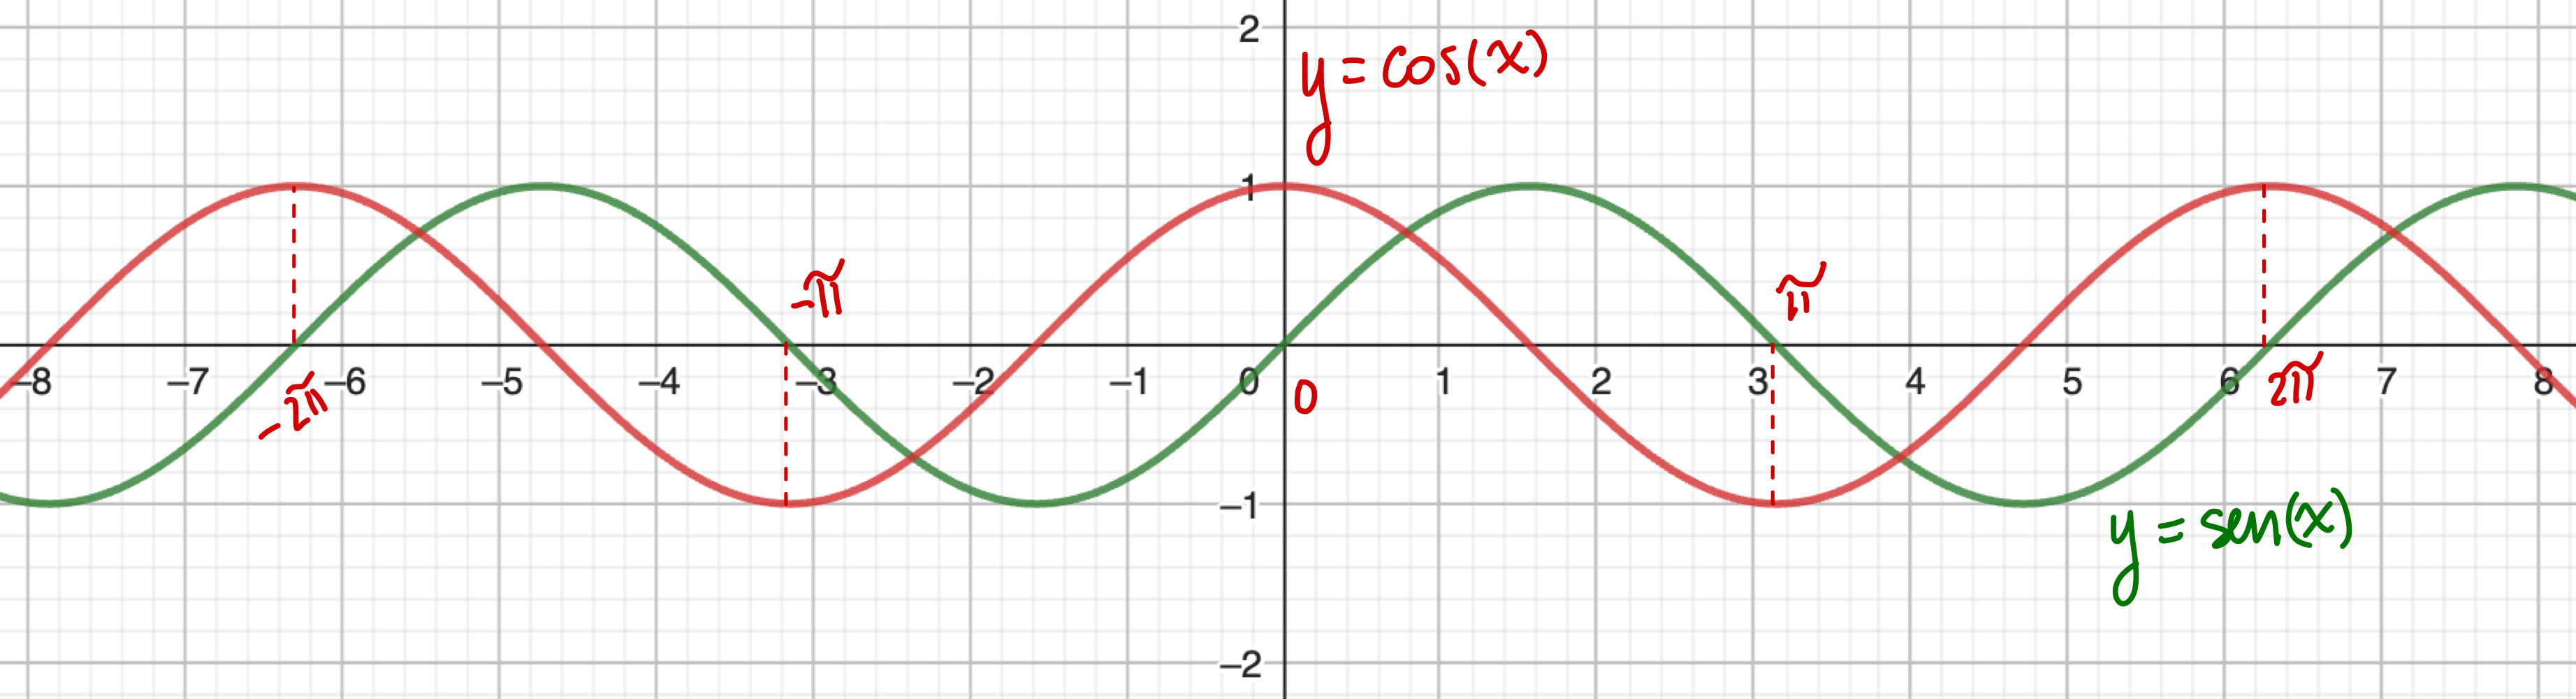
\includegraphics[width=.8\textwidth]{pics/seno-coseno.png}}


Esto que observamos para la función coseno y su derivada, ocurre en general, como lo establece el siguiente teorema.

\begin{theorem}[Teorema de Fermat]
    Si $f$ está definida en el intervalo abierto $(a,b)$ y si $x_0\in(a,b)$ es un punto máximo o un punto mínimo de $f$ donde $f$ es derivable, entonces
    \[
    f'(x_0)=0.
    \]
\end{theorem}

\begin{proof}
    Supongamos que $f$ tiene un mínimo en $x_0$. Entonces
    \[
    f(x)\ge f(x_0), \quad\text{para todo $x\in (a,b)$.}
    \]
    Como $f$ es derivable, existe $\D\limxo \frac{f(x)-f(x_0)}{x-x_0} = f'(x_0)$, y luego
    \[
    f'(x_0) = \limxo \frac{f(x)-f(x_0)}{x-x_0} = \limxop \frac{f(x)-f(x_0)}{x-x_0} = \limxom \frac{f(x)-f(x_0)}{x-x_0}.
    \]
    Si $x>x_0$, entonces $\frac{f(x)-f(x_0)}{x-x_0}\ge 0$ por lo que 
    \[
    f'(x_0) = \limxop \frac{f(x)-f(x_0)}{x-x_0} \ge 0.
    \]
    Si $x<x_0$, entonces $\frac{f(x)-f(x_0)}{x-x_0}\le 0$ por lo que 
    \[
    f'(x_0) = \limxom \frac{f(x)-f(x_0)}{x-x_0} \le 0.
    \]
    Por lo tanto, $0 \le f'(x_0) \le 0$, es decir $f'(x_0)=0$.

    Análogamente se prueba la misma conclusión si $f$ tiene un máximo en $x_0$.
\end{proof}

Observemos que el teorema de Fermat no se puede aplicar si la función está definida sólo sobre un intervalo cerrado $[a,b]$ y alcanza su máximo o mínimo en un extremo.

\medskip
\centerline{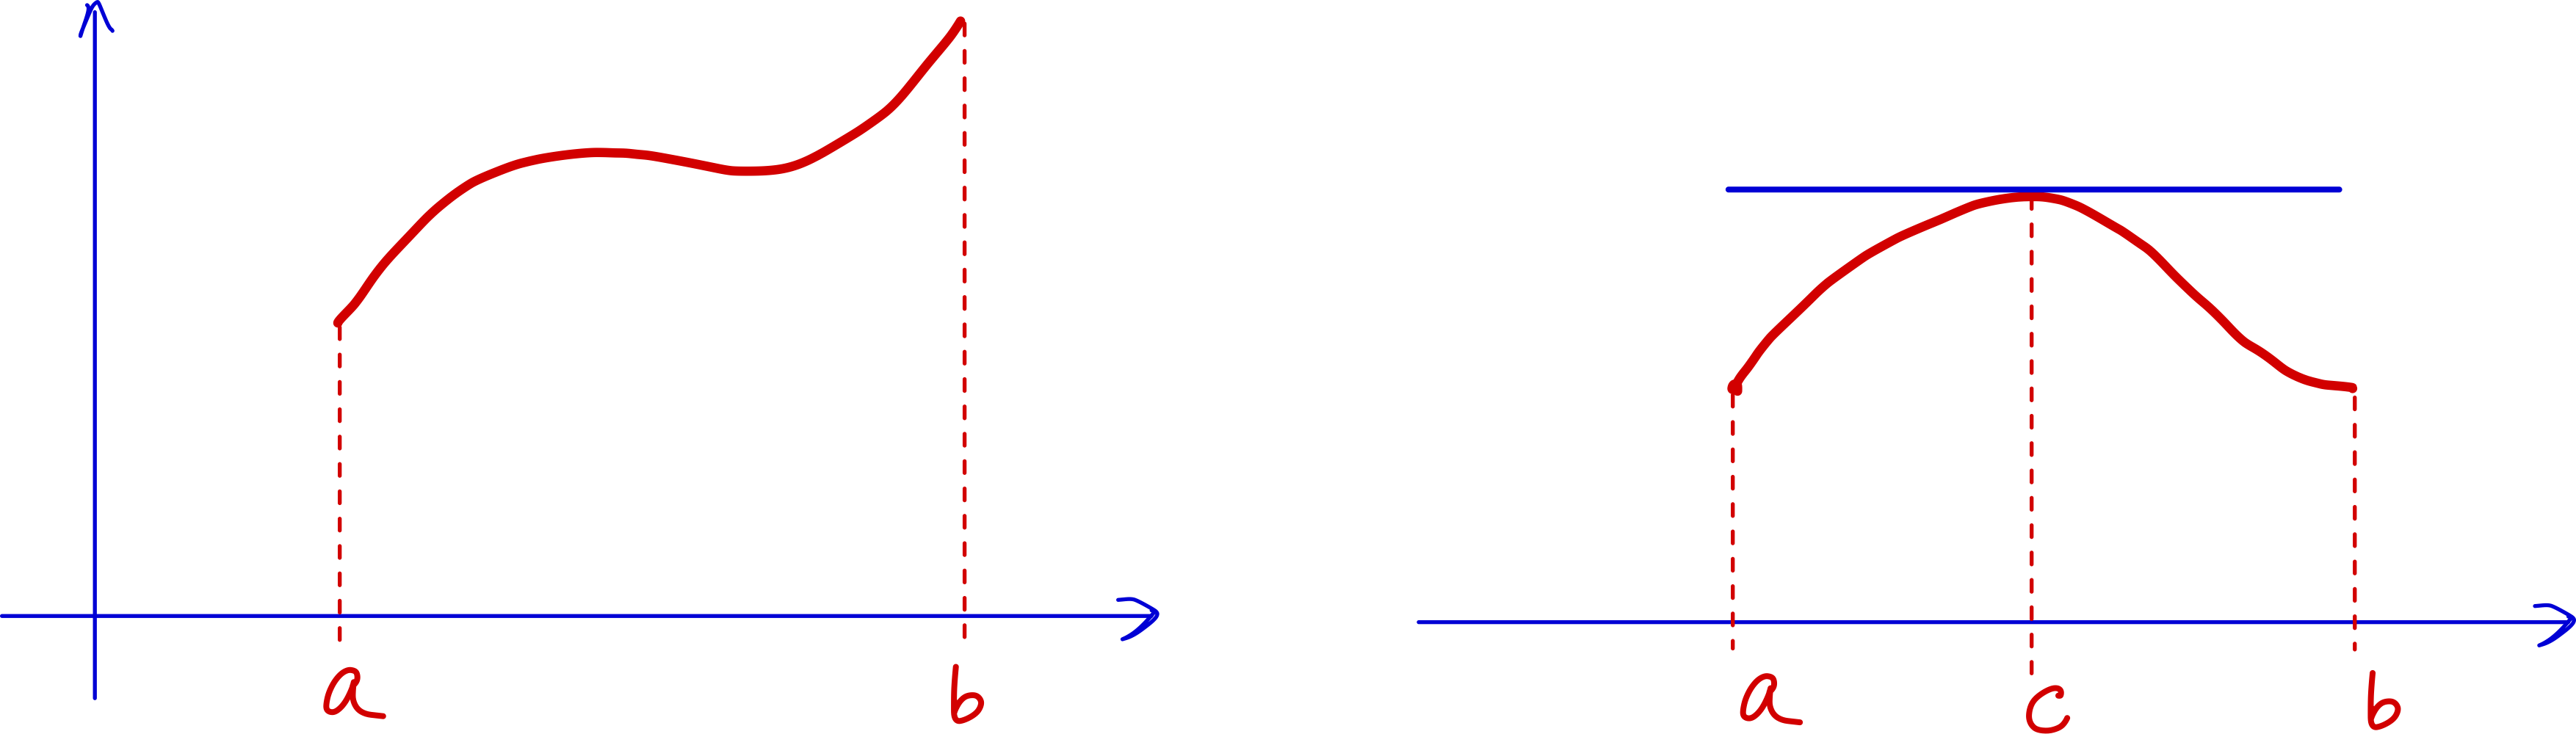
\includegraphics[width=.8\textwidth]{pics/rolle.png}}

Ahora, para funciones definidas en intervalos cerrados, probamos el hecho, geométricamente evidente de que si una función toma el mismo valor en los extremos de un intervalo, entonces, en algún punto intermedio de dicho intervalo, la tangente será horizontal. Más precisamente:

\begin{theorem}[Teorema de Rolle]
    Si $f$ es continua en $[a,b]$, derivable en $(a,b)$ y $f(a)=f(b)$, entonces existe $c\in(a,b)$ tal que $f'(c)=0$.
\end{theorem}

\begin{proof}
    Como $f$ es continua en el intervalo cerrado $[a,b]$, entonces por el Teorema~\ref{T:continua->maximo y minimo} existe $x_1\in[a,b]$ donde $f$ alcanza su mínimo y existe $x_2\in [a,b]$ donde $f$ alcanza su máximo.

Existen diferentes posibilidades:
\begin{itemize}
    \item     Si $x_1\neq a$ y $x_1\neq b$, entonces $x_1\in(a,b)$. Luego, como $f$ es diferenciable en $(a,b)$ y alcanza su mínimo en $x_1\in(a,b)$, el Teorema de Fermat nos dice que $f'(x_1)=0$, y hemos probado el teorema.
    \item  Si $x_2\neq a$ y $x_2\neq b$, entonces $x_2\in(a,b)$. Luego, como $f$ es diferenciable en $(a,b)$ y alcanza su máximo en $x_2\in(a,b)$, el Teorema de Fermat nos dice que $f'(x_2)=0$, y hemos probado el teorema.
    \item Si no ocurre ningúno de los dos casos anteriores, quiere decir que los máximos y mínimos se alcanzan en los extremos del intervalo. Pero en los extremos del intervalo la función toma el mismo valor, luego
    \[
    f(a)=f(b)\le f(x)\le f(a)=f(b), \quad\text{para todo $x\in [a,b]$}.
    \]
    Es decir, la función $f$ es constante en $[a,b]$ y por lo tanto $f'(x)=0$ para todo $x\in(a,b)$.\qedhere
\end{itemize}
\end{proof}

Este fue nuestro primer Teorema del Valor Medio. El segundo, que enunciaremos y probaremos a continuación, tiene también una interpretación geométrica: existe algún punto entre $a$ y $b$ en donde la recta tangente es paralela a la \emph{cuerda} (recta que pasa por $(a,f(a))$ y $(b,f(b))$.

\medskip
\centerline{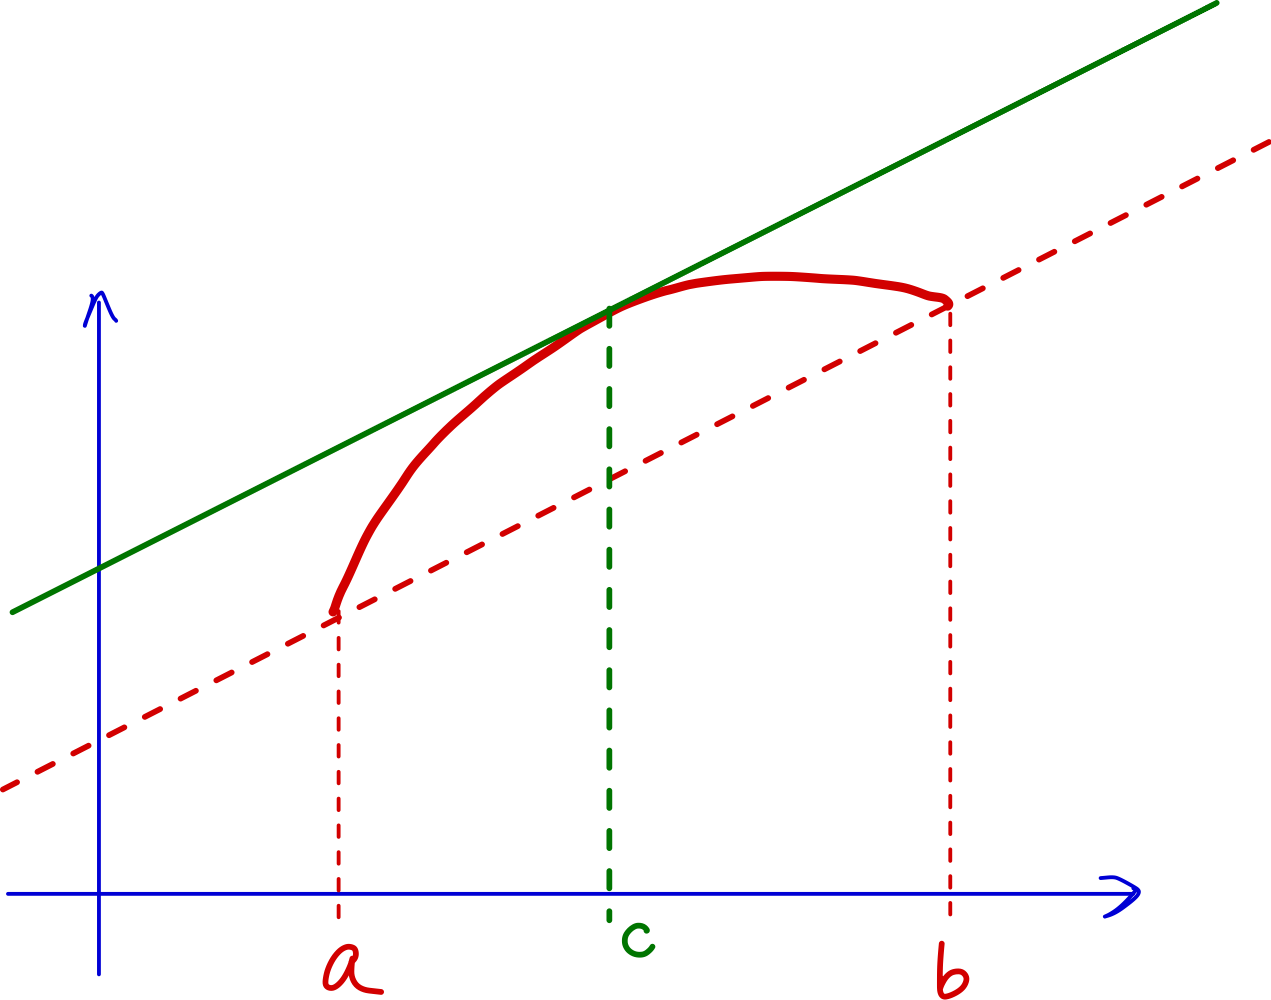
\includegraphics[width=.6\textwidth]{pics/tvm.png}}

\begin{theorem}[Teorema del Valor Medio (de Lagrange)]\label{T:TVM}
       Si $f$ es continua en $[a,b]$ y derivable en $(a,b)$, entonces existe $c\in(a,b)$ tal que 
       \[
       f'(c)=\frac{f(b)-f(a)}{b-a}.
       \]
\end{theorem}

\begin{proof}
    Para demostrar este teorema, consideramos la ecuación de la recta  que pasa por $(a,f(a))$ y $(b,f(b))$:
    \[
    y - f(a) = \frac{f(b)-f(a)}{b-a} (x-a),
    \]
    que puede escribirse también como
    \[    
    y = f(a) + \frac{f(b)-f(a)}{b-a} (x-a).
    \]
    Ahora definimos la función 
    \[
    g(x) = f(x) - \left[ f(a) + \frac{f(b)-f(a)}{b-a} (x-a) \right].
    \]
    Esta función cumple que es continua en $[a,b]$ y derivable en $(a,b)$. Además:
    \begin{align*}
        g(a) &= f(a) - \left[ f(a) + \frac{f(b)-f(a)}{b-a} \underbrace{(a-a)}_0 \right] 
        = f(a)-f(a)=0,
        \\
        g(b) &= f(b) - \left[ f(a) + \frac{f(b)-f(a)}{\cancel{b-a}} \cancel{(b-a)} \right] 
        = f(b)-\left[f(a)+f(b)-f(a)\right] = 0.
    \end{align*}
    Por lo tanto, $g(a)=g(b)=0$ y $g$ cumple las hipótesis del Teorema de Rolle, y luego existe $c\in(a,b)$ tal que $g'(c)=0$. 
    Si calculamos la derivada de $g$, vemos que
    \[
    g'(x) = f'(x) - \frac{f(b)-f(a)}{b-a} \cdot 1,
    \]
    y luego 
    \[
    0 = g'(c) = f'(c) - \frac{f(b)-f(a)}{b-a} ,
    \]
    que inmediatamente implica lo que queríamos demostrar.
\end{proof}

Pasamos ahora a probar consecuencias del Teorema del Valor Medio.

En primer lugar, recordemos que la derivada de una función constante es la función nula.
Nos planteamos la pregunta recíproca. Si una función tiene derivada nula en todo punto: ?`Es esa función necesariamente constante?
La respuesta es efectivamente afirmativa:

\begin{proposition}
    Si $f$ es continua en $[a,b]$, derivable en $(a,b)$ y $f'(x)=0$, para todo $x\in(a,b)$, entonces % existe $k\in\R$ tal que 
    \[ 
    f(x)=f(a), \quad\text{para todo $x\in [a,b]$}.
    \]
\end{proposition}

\begin{proof}
    Sea $x_0 \in (a,b]$. Luego $[a,x_0]\subset [a,b]$ y resulta que $f$ es continua en $[a,x_0]$ y derivable en $(a,x_0)$. Entonces cumple las hipótesis del Teorema del valor medio en el intervalo $[a,x_0]$, por lo tanto, existe $c\in [a,x_0]$ tal que 
    \[
    f'(c) = \frac{f(x_0)-f(a)}{x_0-a}.
    \]
    Pero $f'(c)=0$ por lo que $f(x_0)-f(a)=0$ que a su vez implica $f(x_0)=f(a)$. Con esto concluye nuestra demostración.
\end{proof}

\begin{corollary}
    Si $f$ y $g$ son continuas en $[a,b]$, derivables en $(a,b)$ y $f'(x)=g'(x)$, para todo $x\in(a,b)$, entonces existe $k\in\R$ tal que 
    \[ 
    f(x)=g(x)+k, \quad\text{para todo $x\in [a,b]$}.
    \]
\end{corollary}

\begin{proof}
    Definimos $h(x)=f(x)-g(x)$. Luego 
    \[
    h'(x)=f'(x)-g'(x)=0, \quad\text{para todo $x\in [a,b]$}.
    \]
    Entonces $f(x)-g(x)=f(a)-g(a)$, para todo $x\in[a,b]$. 
    Llamando $k=f(a)-g(a)$ se obtiene el resultado deseado.
\end{proof}

El siguiente resultado es una consecuencia importante del Teorema del Valor Medio, que nos permite deducir información de $f$ a partir de información sobre su derivada $f'$.

\begin{proposition}\label{P:signo-derivada=>tendencia}
    Sea $f$ una función continua en $[a,b]$ y derivable en $(a,b)$:
    \begin{enumerate}
        \item Si $f'(x)>0$ para todo $x\in(a,b)$, entonces $f$ es estrictamente creciente en $[a,b]$, 
        es decir, si $a\le x_1<x_2\le b$, entonces $f(x_1)<f(x_2)$.
        \item Si $f'(x)<0$ para todo $x\in(a,b)$, entonces $f$ es estrictamente decreciente en $[a,b]$,
        es decir, si $a\le x_1<x_2\le b$, entonces $f(x_1)>f(x_2)$.
    \end{enumerate}
\end{proposition}

\begin{proof}
    \begin{enumerate}
        \item Sean $x_1,x_2\in[a,b]$ con $x_1<x_2$, es decir, $a\le x_1<x_2\le b$. Consideramos $f$ sobre el intervalo $[x_1,x_2]$ resulta que $f$ es continua en ese intervalo y derivable en $(x_1,x_2)$. Es decir, satisface las hipótesis del Teorema del Valor Medio (Teorema~\ref{T:TVM}) en el intervalo $[x_1,x_2]$.
        Por lo tanto, existe $c\in(x_1,x_2)$ tal que 
        \[
        \frac{f(x_2)-f(x_1)}{x_2-x_1} = f'(c).
        \]
        O sea,
        \[
        f(x_2)-f(x_1) = f'(c)\, (x_2-x_1).
        \]
        Pero $f'(c)>0$, por lo que $f(x_2)-f(x_1)>0$, o lo que es lo mismo, $f(x_2)>f(x_1)$.
        
        \item Se prueba de la misma manera, sólo que ahora $f'(c)<0$ y por lo tanto $f(x_2)-f(x_1)<0$, que es lo mismo que decir $f(x_2)<f(x_1)$.
    \end{enumerate}
\end{proof}

Presentamos ahora un teorema importante que nos va a servir para calcular las derivadas de más funciones.

\begin{theorem}[Derivada de la función inversa]
    Sea $f$ una función continua y estrictamente creciente, o estrictamente decreciente en $[a,b]$ (con lo cual existe inversa):
    \begin{itemize}
        \item $\D f^{-1}:[f(a),f(b)]\to [a,b]$ cuando $f$ es estrictamente creciente;
        \item $\D f^{-1}:[f(b),f(a)]\to [a,b]$ cuando $f$ es estrictamente decreciente.
    \end{itemize}
    Si $x\in(a,b)$ es un punto tal que $f$ es derivable en $x$, y $f'(x)\neq 0$, entonces $f^{-1}$ es derivable en $y=f(x)$ y además:
    \[
    \big(f^{-1}\big)'(y) = \frac1{f'(x)},
    \]
    que también podemos escribir así:
    \begin{equation}\label{eq:derivada inversa}
    \big(f^{-1}\big)'(f(x)) = \frac1{f'(x)},
    \qquad\text{o}\qquad
    \big(f^{-1}\big)'(y) = \frac1{f'(f^{-1}(y))},
    \end{equation}
\end{theorem}

\begin{proof}
    La demostración se verá en la clase de \emph{Coloquio de Demostraciones}.
\end{proof}

Si bien esta demostración es un poco complicada, la parte complicada es demostrar que $f\inv$ es derivable. Suponiendo que es derivable, la fórmula es sencilla a partir de la regla de la cadena. En efecto, por definición de función inversa, $f\circ f\inv(y) = y$, luego, por un lado
\[
\frac{d (f\circ f\inv)(y)}{dy} = \frac{dy}{dy} = 1,
\]
y por otro lado, usando la regla de la cadena,
\[
    \frac{d (f\circ f\inv)(y)}{dy} = f'\big(f\inv(y)\big)\cdot (f\inv)'(y).
\]
Luego,
\[
    f'\big(f\inv(y)\big)\cdot (f\inv)'(y)=1
    \quad\implies\quad  (f\inv)'(y)= \frac1{f'\big(f\inv(y)\big)}.
\]

\begin{example}
    Consideremos la función $f:\R\to\R$ dada por $f(x)=\sen x$. 
    Su derivada es $f'(x)=\cos x$, que es positiva en el intervalo $-\frac\pi2<x<\frac\pi2$.
    Luego, el seno es una función estrictamente creciente en $[-\pi/2,\pi/2]$ y como además es continua, existe función inversa 
    \[
    \arcsen: [-1,1] \to \Big[-\frac\pi2,\frac\pi2\Big]:
    \qquad
    \arcsen y = x \quad\iff\quad \sen x = y.
    \]

    \centerline{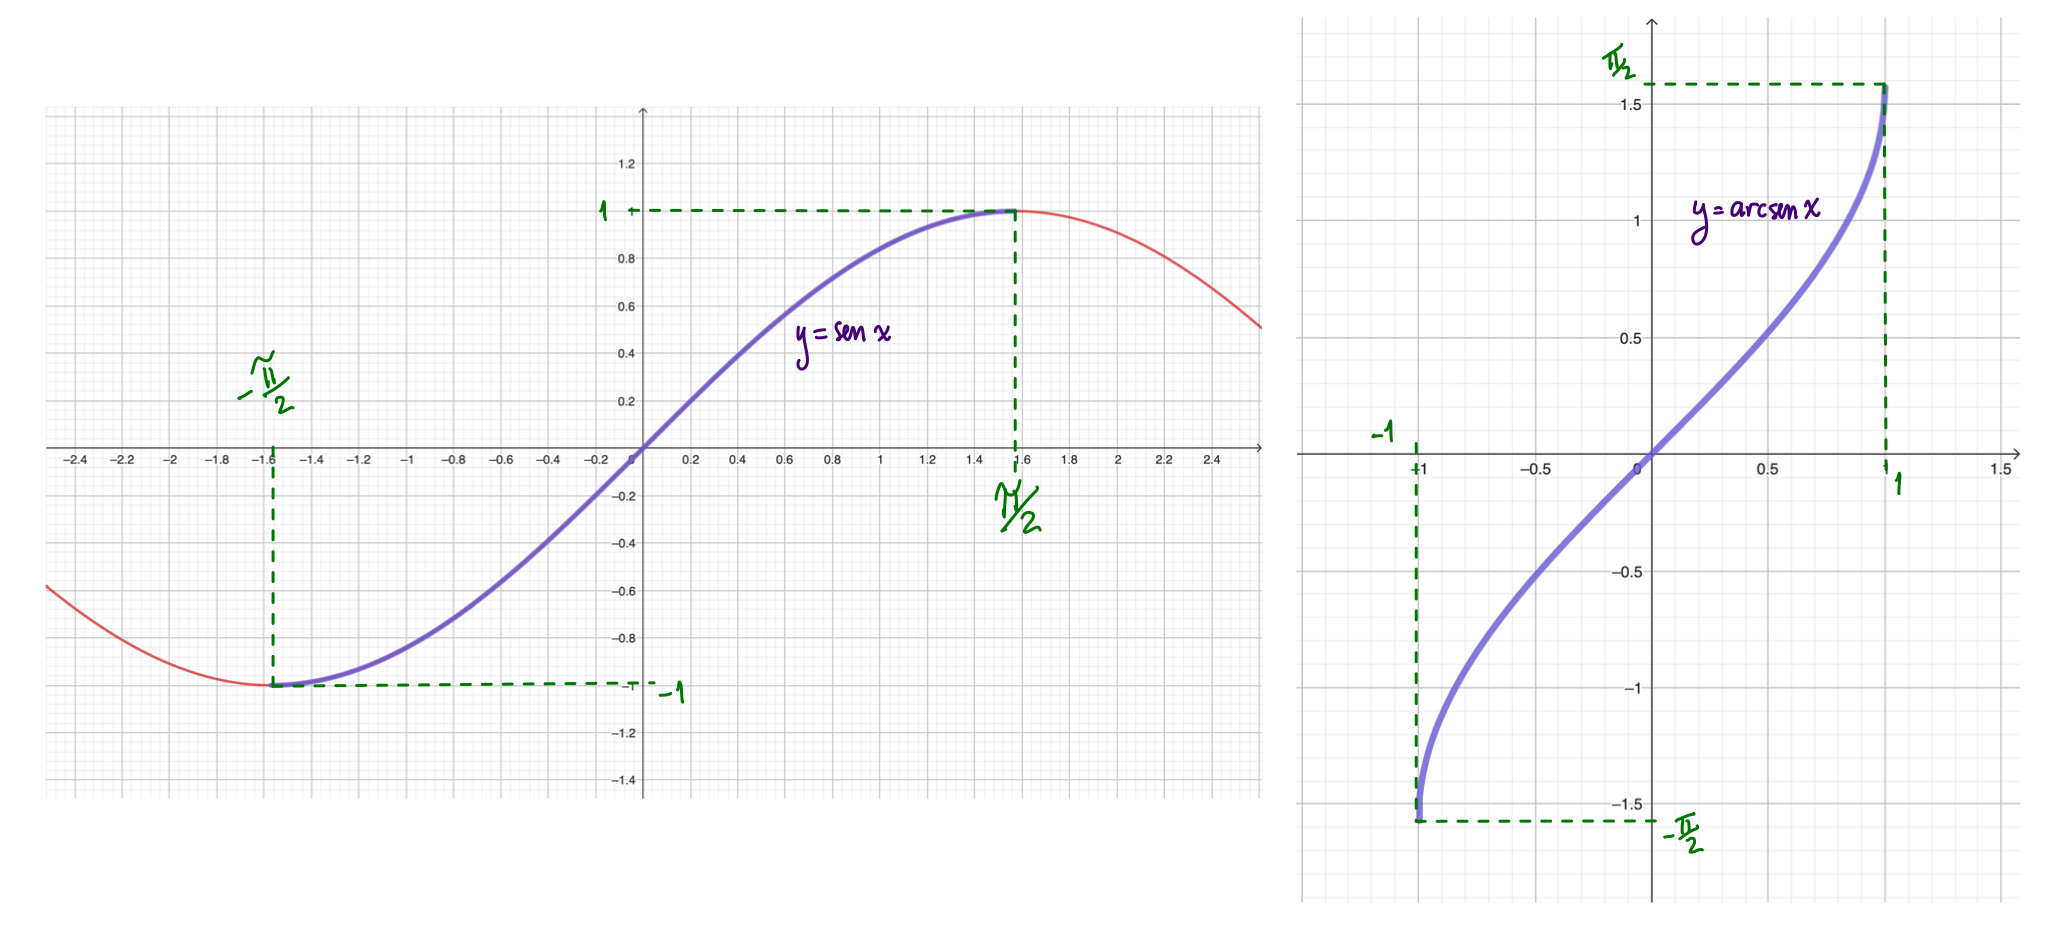
\includegraphics[width=.8\textwidth]{pics/seno-arcseno.jpeg}}
    
    Como $\sen'(x)=\cos(x)\neq 0$ en $\big(-\frac\pi2,\frac\pi2\big)$, entonces $\arcsen$ es derivable en $(-1,1)$.
    Para hallar su derivada, usamos la segunda fórmula de~\eqref{eq:derivada inversa}:
    \[
    \arcsen'(y) = \frac{1}{\sen'(\arcsen y)}
    = \frac1{\cos(\arcsen y)} = \frac1{\cos x},
    \]
    donde $x=\arcsen y$. Entonces $\sen x=y$, y tenemos que deducir cuánto vale $\cos x$ sabiendo que $\sen x = y$. Para esto, utilizaremos que
    \[
    \cos^2 x + \sen^2 x = 1,\qquad\text{y}\qquad x\in\big(-\frac\pi2,\frac\pi2\big).
    \]
    De la primera deducimos que $\cos x = \pm \sqrt{1-y^2}$, como $x\in\big(-\frac\pi2,\frac\pi2\big)$ deducimos que $\cos x > 0$ por lo que $\cos x = \sqrt{1-y^2}$. Luego
    \[
    \arcsen'(y) = \frac1{\sqrt{1-y^2}}, \qquad \text{para $y\in (-1,1)$}.
    \]
\end{example}

\begin{example}
    Consideremos ahora la función $f:\R\to\R$ dada por $f(x)=\cos x$. 
    Su derivada es $f'(x)=-\sen x$, que es negativa en el intervalo $0<x<\pi$.
    Luego, el coseno es una función estrictamente decreciente en $[0,\pi]$ y como además es continua, existe función inversa 
    \[
    \arccos: [-1,1] \to [0,\pi]:
    \qquad
    \arccos y = x \quad\iff\quad \cos x = y.
    \]

    \centerline{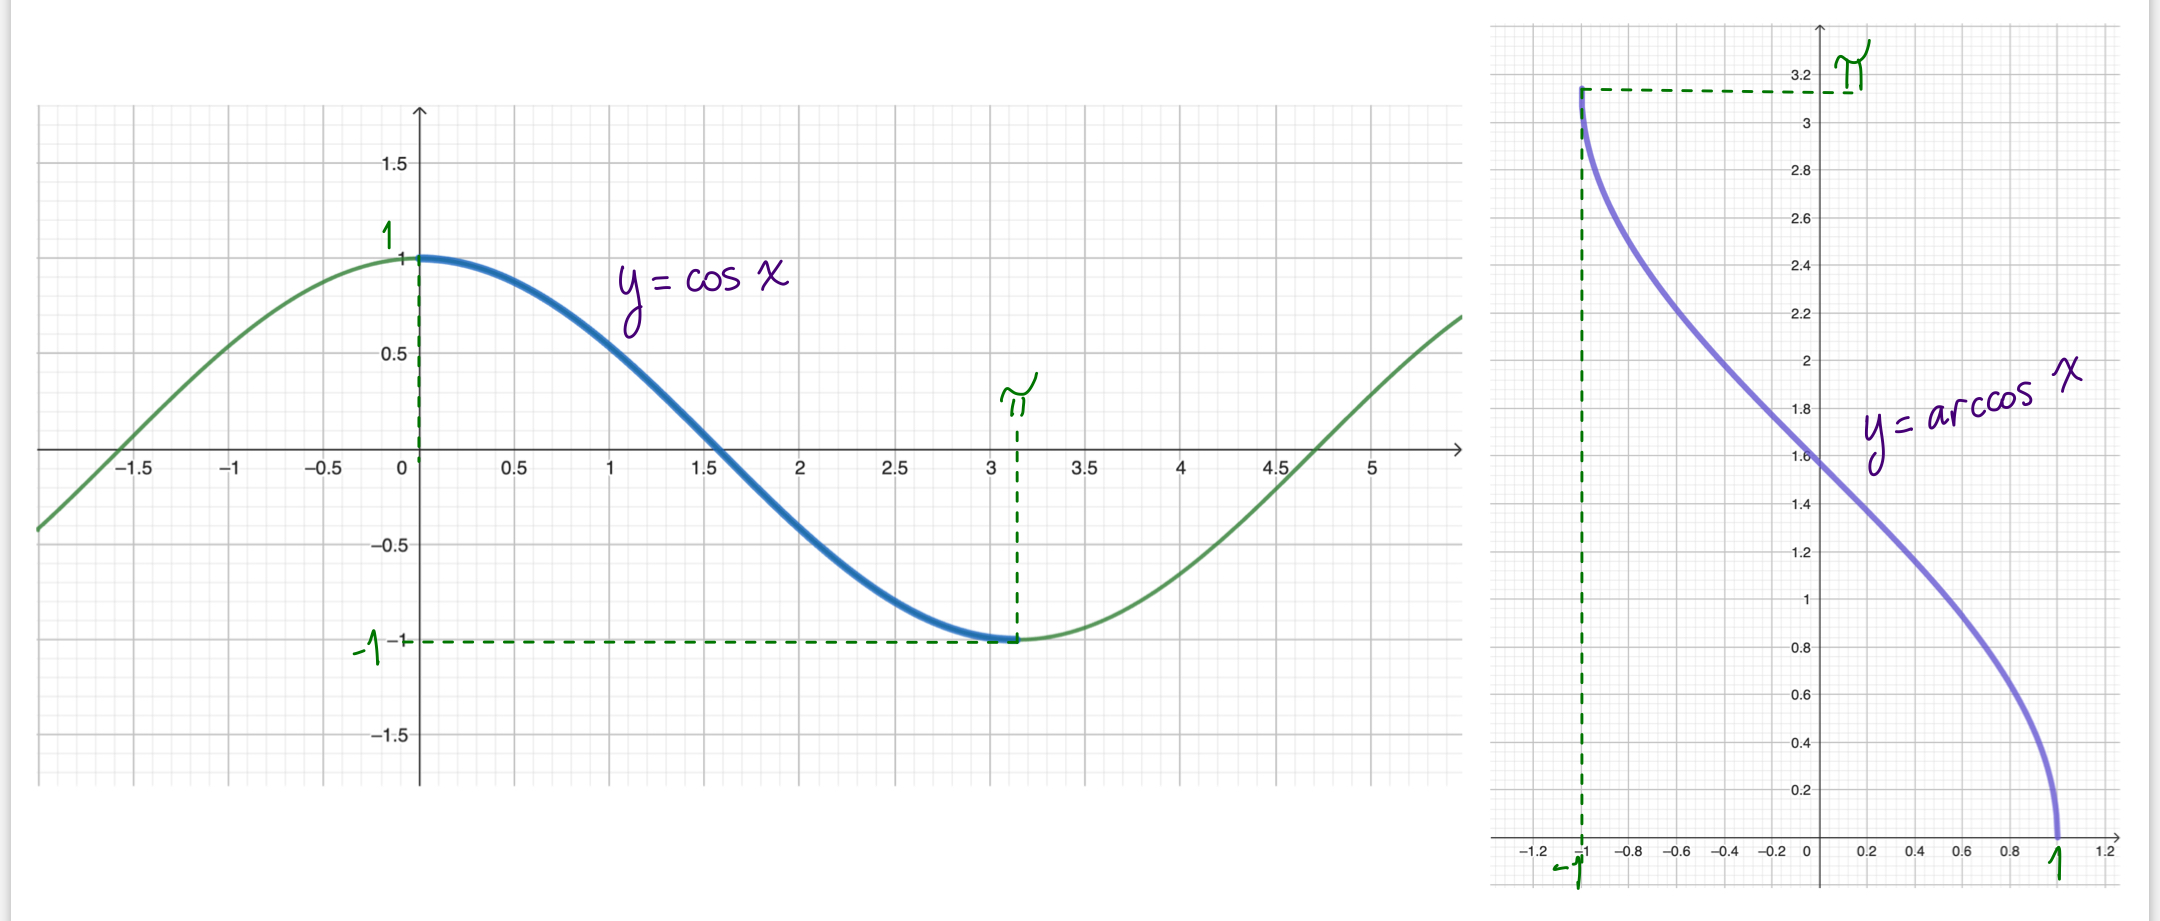
\includegraphics[width=.8\textwidth]{pics/cos-arccos.jpeg}}
    
    Como $\cos'(x)=-\sen(x)\neq 0$ en $(0,\pi)$, entonces $\arccos$ es derivable en $(-1,1)$.
    Para hallar su derivada, usamos la segunda fórmula de~\eqref{eq:derivada inversa}:
    \[
    \arccos'(y) = \frac{1}{\cos'(\arccos y)}
    = -\frac1{\sen(\arccos y)} = -\frac1{\sen x},
    \]
    donde $x=\arccos y$. Entonces $\cos x=y$, y tenemos que deducir cuánto vale $\sen x$ sabiendo que $\cos x = y$. Para esto, utilizaremos que
    \[
    \cos^2 x + \sen^2 x = 1,\qquad\text{y}\qquad x\in(0,\pi).
    \]
    De la primera deducimos que $\sen x = \pm \sqrt{1-y^2}$, como $x\in(0,\pi)$ deducimos que $\sen x > 0$ por lo que $\sen x =  \sqrt{1-y^2}$. Luego
    \[
    \arccos'(y) = -\frac1{\sqrt{1-y^2}}, \qquad \text{para $y\in (-1,1)$}.
    \]
\end{example}

Veamos un último ejemplo:

\begin{example}
    Consideremos ahora la función dada por $\D f(x)=\tan x=\frac{\sen x}{\cos x}$, cuyo dominio es todo $\R$ excepto los puntos de la forma $\frac\pi2+n\pi$, $n\in\Z$, que son los puntos donde se anula el denominador $\cos x$.
    Quedó como ejercicio en una de las secciones anteriores calcular $\tan'(x)$, y la respuesta era
    \[
    \tan'(x)=\frac1{\cos^2x}.
    \]
    Esta derivada es siempre positiva, por lo tanto, $f(x)$ es estrictamente creciente en cada intervalo de la forma $(n\pi-\frac\pi2,n\pi+\frac\pi2)$. Consideremos esta función en el intervalo $(-\frac\pi2,\frac\pi2)$, donde es estrictamente creciente. Observamos que
    \[
    \lim_{x\to-\frac\pi2^+}\tan(x)=-\infty,
    \qquad\text{y}\qquad
    \lim_{x\to\frac\pi2^-}\tan(x)=+\infty.
    \]
    Por lo tanto, la función tangente es biyectiva de $(-\frac\pi2,\frac\pi2)$ en $(-\infty,+\infty)$, y existe función inversa 
    \[
    \arctan: \R \to \Big(-\frac\pi2,\frac\pi2\Big)
    \qquad
    \arctan y = x \quad\iff\quad \tan x = y.
    \]

    \centerline{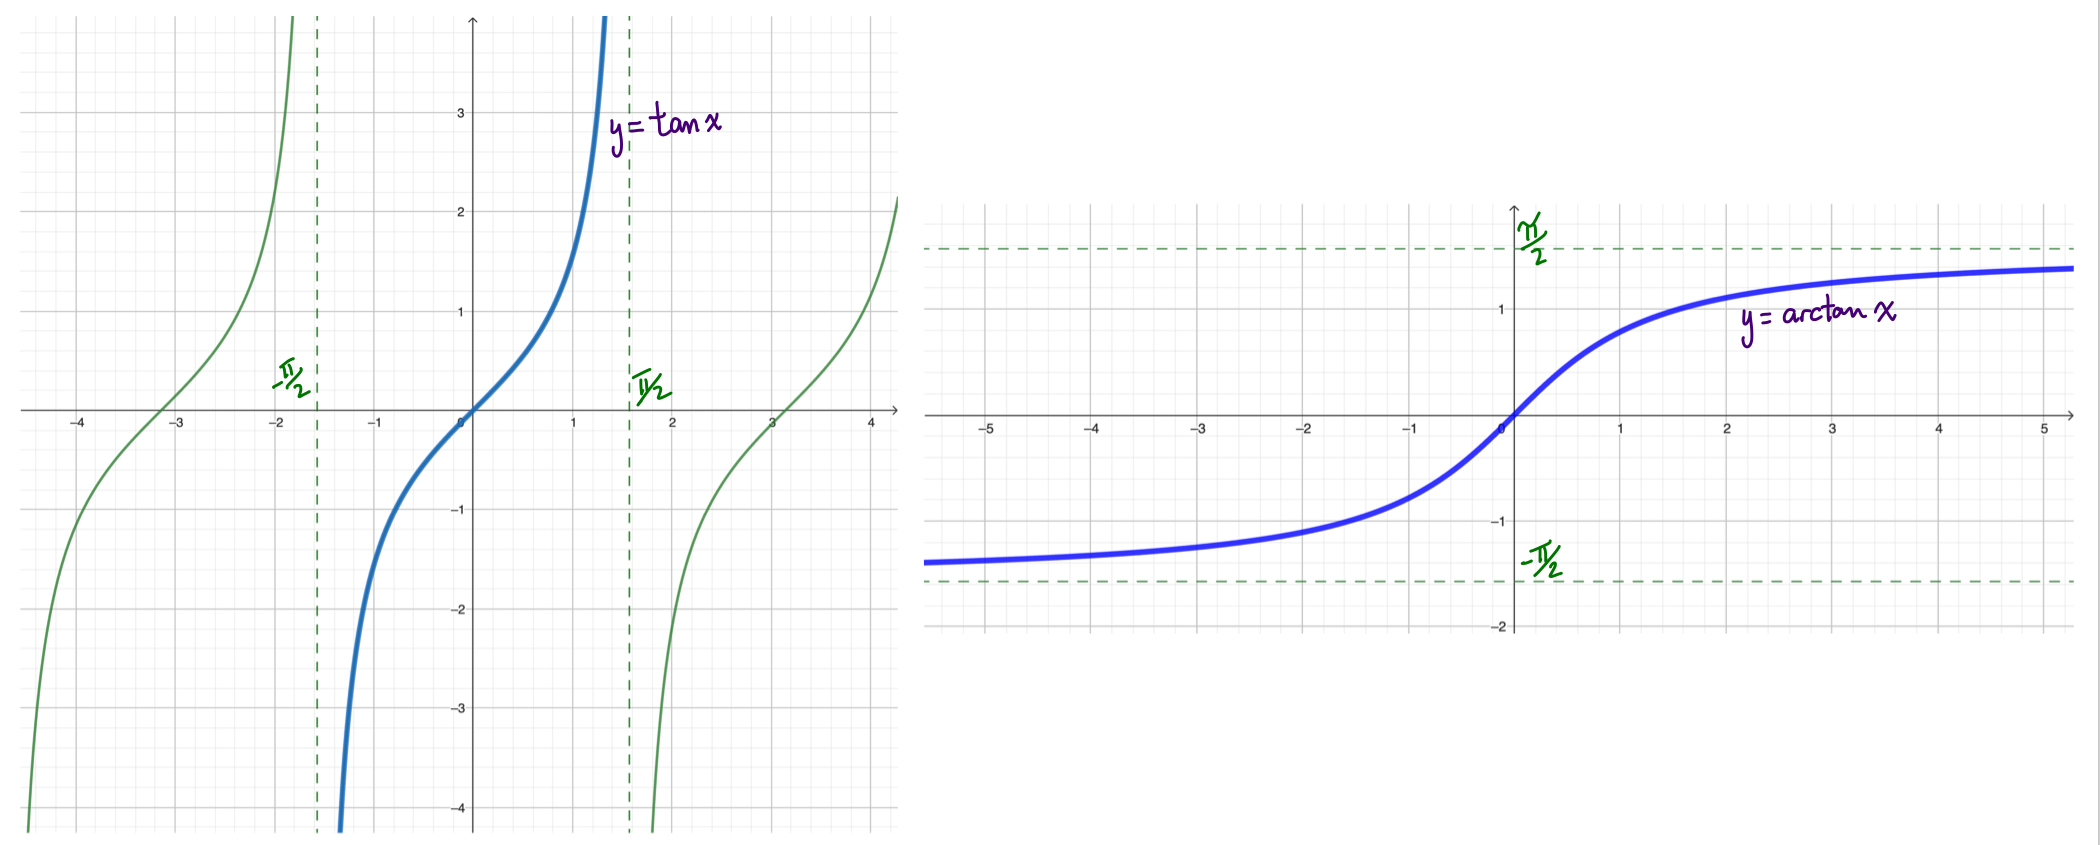
\includegraphics[width=.8\textwidth]{pics/tan-atan.jpeg}}
    
 Como $\tan'(x)=\frac1{\cos^2(x)}> 0$ en $(-\frac\pi2,\frac\pi2)$, entonces $\arctan$ es derivable en $\R$.
    Para hallar su derivada, usamos la segunda fórmula de~\eqref{eq:derivada inversa}:
    \[
    \arctan'(y) = \frac{1}{\tan'(\arctan y)}
    = \frac1{\frac1{\cos^2(\arctan y)}} 
    = \cos^2(\arctan y)
    = \cos^2 x,
    \]
    donde $x=\arctan y$. Entonces $\tan x=y$, y tenemos que deducir cuánto vale $\cos^2 x$ sabiendo que $\tan x = y$. 
    Veamos
    \begin{align*}
        \frac{\sen x}{\cos x} = y
        &\implies
        \frac{\sen^2 x}{\cos^2 x} = y^2
        \implies 
        \frac{1-\cos^2 x}{\cos^2 x} = y^2
        \\
        &\implies
        1-\cos^2 x = y^2 \, \cos^2x
        \implies 
        1 = \cos^2 x + y^2 \, \cos^2x
        = \cos^2 x \, \big(1+y^2\big)
        \\
        &\implies \cos^2x = \frac1{1+y^2}.
    \end{align*}
    De aquí obtenemos que
    \[
    \arctan'(y) =  \frac1{1+y^2},
    \quad\text{para todo $y\in\R$.}
    \]
\end{example}


\subsubsection*{Ejercicios de la sección~\getcurrentref{chapter}.\getcurrentref{section}}

\begin{enumerate}
\item * Si $f:\R\to\R$ es continua en $\R$ y derivable en todo punto de $\R\setminus\{a\}$, y existe $\D\lim_{x\to a}f'(x)= \ell$, entonces $f$ es derivable en $x=a$ y $f'(a) = \ell$.
Usar el Teorema del Valor Medio (de Lagrange) para calcular las derivadas laterales.

\item Probar las siguientes afirmaciones para una función $f:[a,b]\to \R$ continua en $[a,b]$ y derivable en $(a,b)$:
\begin{enumerate}
  \item Si $f'(x)\ge 0$ para todo $x\in(a,b)$, entonces $f$ es creciente en $[a,b]$; es decir, $a\le x_1<x_2\le b$ implica $f(x_1)\le f(x_2)$.
  \item Si $f$ es creciente, entonces $f'(x)\ge 0$ para todo $x\in(a,b)$.
  \item Si $f'(x)\le 0$ para todo $x\in(a,b)$, entonces $f$ es decreciente en $[a,b]$; es decir, $a\le x_1<x_2\le b$ implica $f(x_1)\ge f(x_2)$
  \item Si $f$ es decreciente, entonces $f'(x)\le 0$ para todo $x\in(a,b)$.
\end{enumerate}

\item Encontrar un ejemplo de una función $f:\R\to\R$ que sea estrictamente creciente y derivable, pero que no cumpla que $f'(x)>0$, para todo $x\in\R$.

\item Probar que la función $f(x)=\sqrt[3]{(x-3)^2}$ satisface $f(1)=f(5)$ pero no existe $c\in(1,5)$ tal que $f'(c)=0$. ?`Por qué no se puede aplicar el Teorema de Rolle?

\item Sea $f(x)=(x-1)\, x\, (x+2)\, (x+5)$. Probar que $f'(x)$ tiene tres raíces reales.

\item Para cada una de las siguientes funciones, determinar el punto $c\in(0,1)$ que cumple el Teorema del Valor Medio en el intervalo $[0,1]$:
\begin{multicols}{3}
  \begin{enumerate}
    \item $f(x)=3x$;
    \item $f(x)=2x^2$;
    \item $f(x)=\sqrt[3]{x}$.
  \end{enumerate}
\end{multicols}

\item Hallar $f'(x)$ para:
\begin{multicols}{2}

  \begin{enumerate}
    \item $\D f(x) = \arcsen(\sqrt x)$;
    \item $\D f(x) = \arccos(x^2+1)$;
    \item $\D f(x) = \big(e^{\arcsen (1/x)}\big)^x$;
    \item $\D f(x) = \sqrt[3]{\arccos\Big(\frac{x^2}{1+x^2}\Big)}$;
    \item $\D f(x) = \ln\big(\arccos (x)\big)$;
  \end{enumerate}
  
\end{multicols}
\end{enumerate}

\section{Máximos y mínimos locales}

\begin{definition}
    Consideremos una función $f:I\to \R$, donde $I$ es un intervalo.
    Decimos que $f$ tiene un \emph{máximo local en $x_0$} cuando existe $\delta>0$ tal que
    \[
    f(x_0)\ge f(x), \quad\text{para todo $x$ en $(x_0-\delta,x_0+\delta)\cap I$}.
    \]
    Decimos que $f$ tiene un \emph{mínimo local en $x_0$} cuando existe $\delta>0$ tal que
    \[
    f(x_0)\le f(x), \quad\text{para todo $x$ en $(x_0-\delta,x_0+\delta)\cap I$}.
    \]
\end{definition}

\begin{figure*}[htbp]
    \centerline{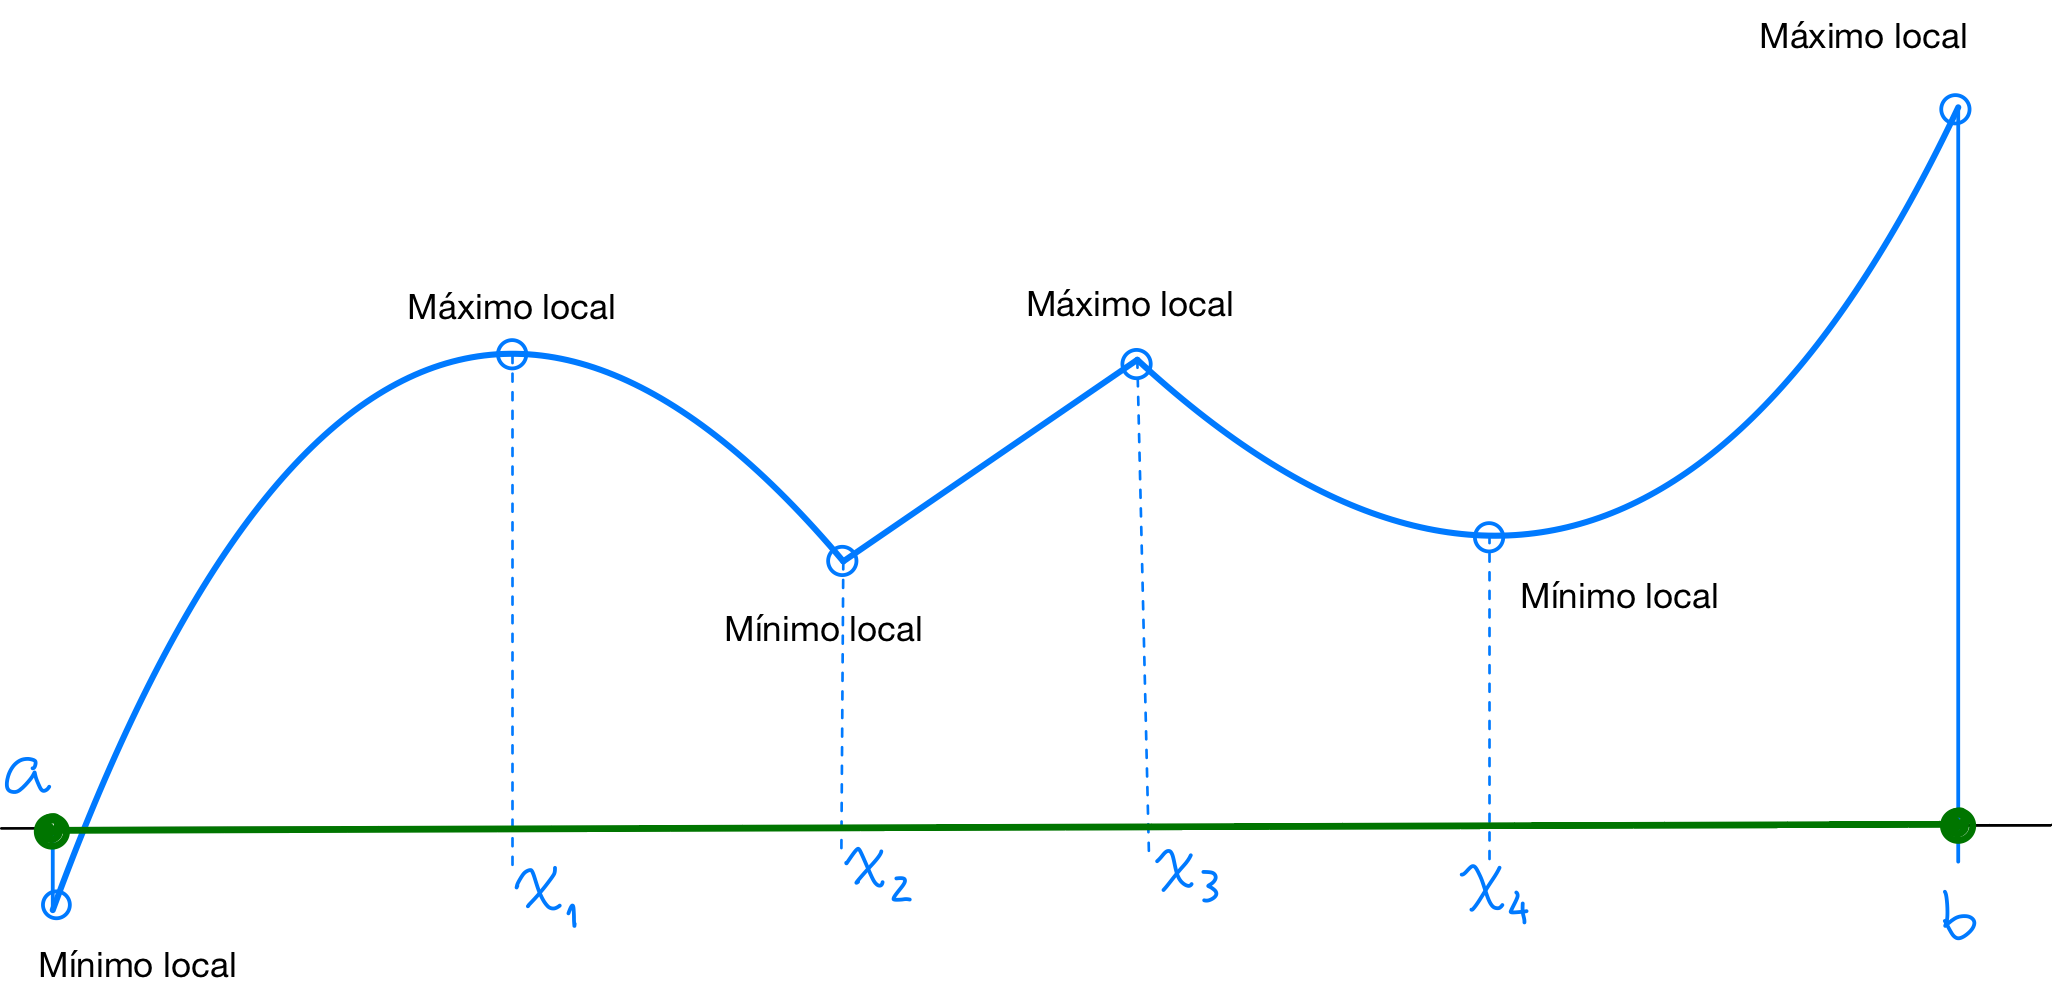
\includegraphics[width=.8\textwidth]{pics/max-min-locales-int-cerrado.png}}
\caption{Máximos y mínimos locales en un intervalo cerrado.}
\end{figure*}

Observamos lo siguiente, con respecto a los máximos y mínimos de una función $f$ en un intervalo cerrado $[a,b]$:
\begin{itemize}
    \item Si $f$ es creciente en un intervalo $[a,a+\delta]$, para algún $\delta>0$, entonces $f(a)$ es un mínimo local de $f$.
    \item Si $f$ es decreciente en un intervalo $[a,a+\delta]$, para algún $\delta>0$, entonces $f(a)$ es un máximo local de $f$.
    \item Si $f$ es creciente en un intervalo $[b-\delta,b]$, para algún $\delta>0$, entonces $f(b)$ es un máximo local de $f$.
    \item Si $f$ es decreciente en un intervalo $[b-\delta,b]$, para algún $\delta>0$, entonces $f(b)$ es un mínimo local de $f$.
    \item Si $x_0\in(a,b)$ y $f$ es decreciente en $[x_0-\delta,x_0]$ y creciente en $[x_0,x_0+\delta]$, para algún $\delta>0$, entonces $f$ tiene un mínimo local en $x_0$.
    \item Si $x_0\in(a,b)$ y $f$ es creciente en $[x_0-\delta,x_0]$ y decreciente en $[x_0,x_0+\delta]$, para algún $\delta>0$, entonces $f$ tiene un máximo local en $x_0$.
\end{itemize}

\begin{figure*}[htbp]
    \centerline{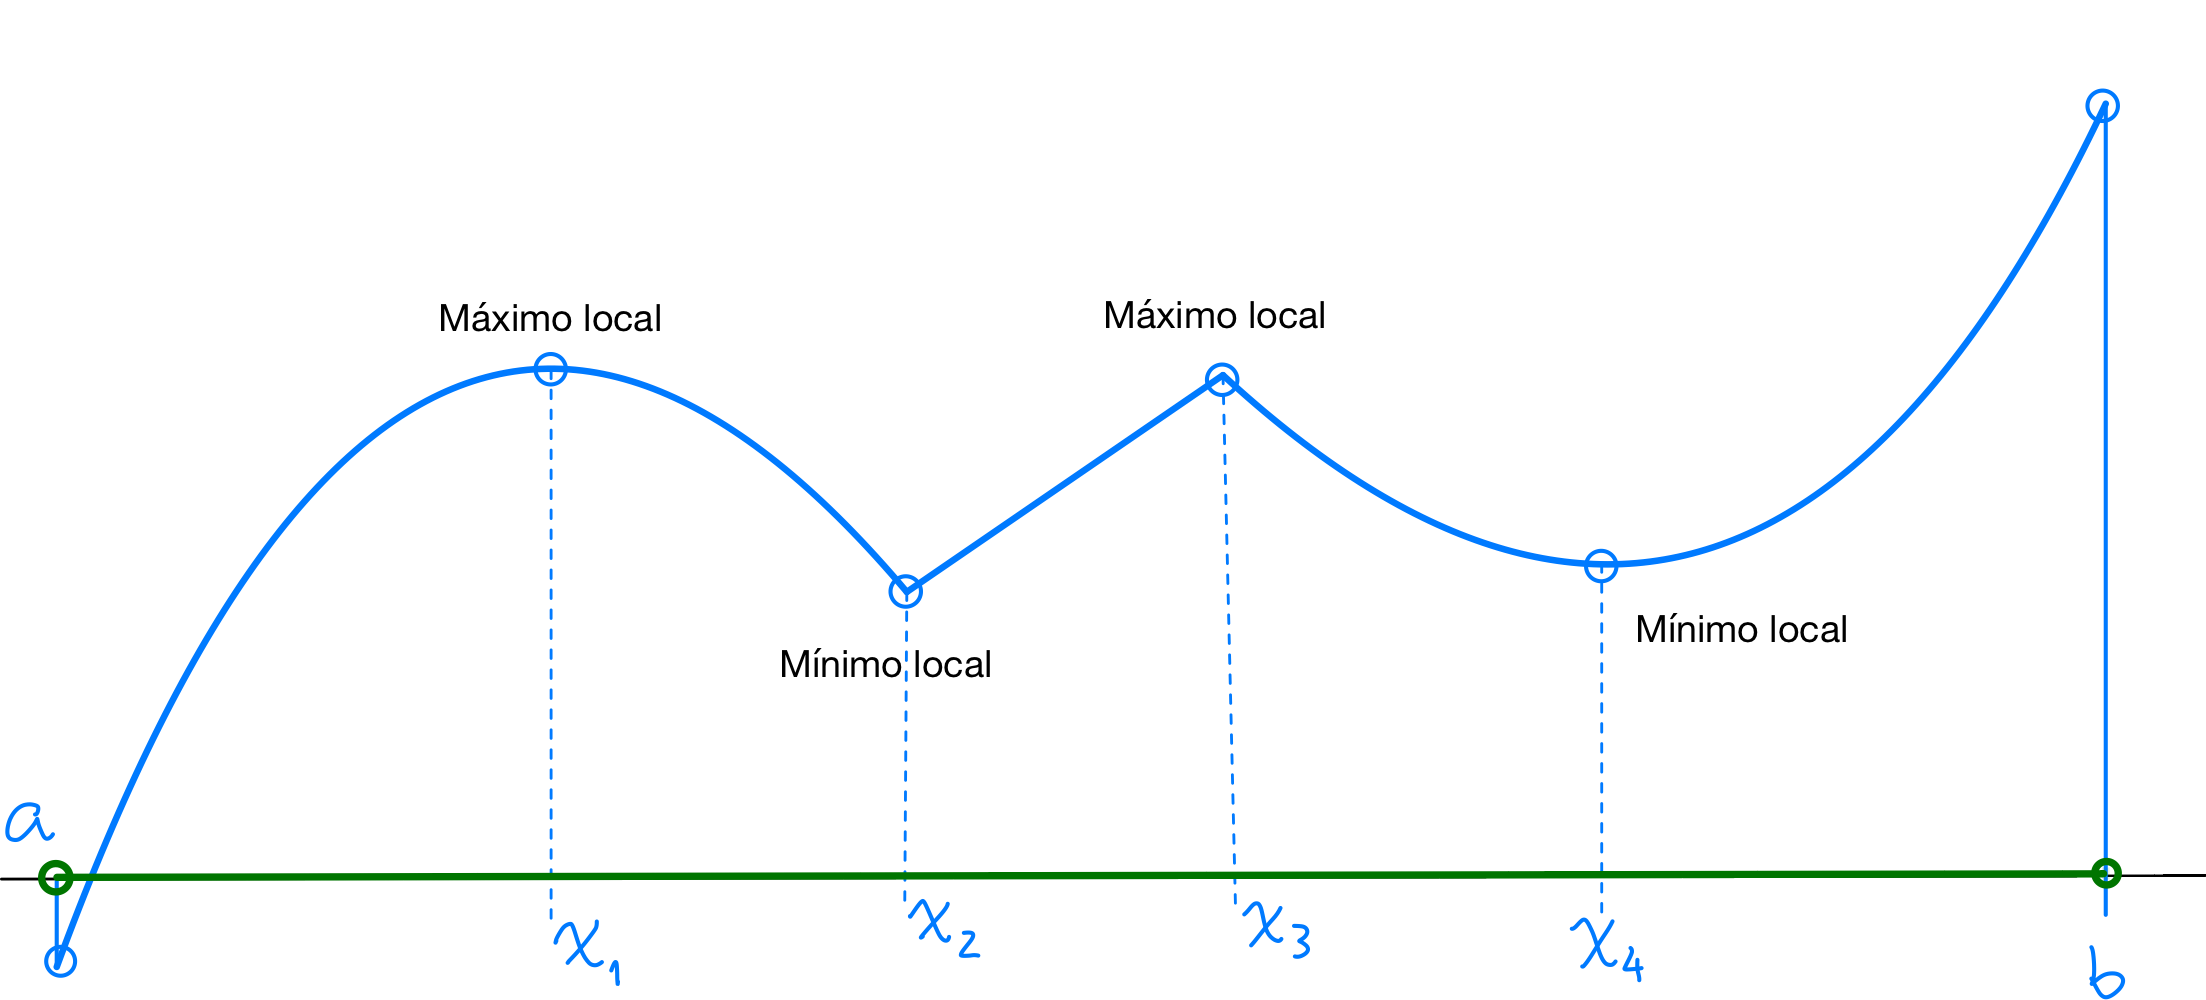
\includegraphics[width=.8\textwidth]{pics/max-min-locales-int-abierto.png}}
\caption{Máximos y mínimos locales en un intervalo abierto.}
\end{figure*}


A continuación vemos un teorema que nos permite determinar los puntos \emph{candidatos} a puntos máximos o mínimos.

\begin{theorem}
    Sea $f:I\to\R$. Si $f$ tiene un máximo o un mínimo local en $x_0$, entonces ocurre una de las tres siguientes:
    \begin{itemize}
        \item $x_0$ es un extremo del intervalo;
        \item $f'(x_0)$ no existe;
        \item $f'(x_0)=0$.
    \end{itemize}
\end{theorem}

\begin{proof}
    Supongamos que $f$ tiene un máximo local en $x_0$ que no es un extremo del intervalo y que $f'(x_0)$ existe; si $x_0$ es un extremo del intervalo o $f'(x_0)$ no existe, no hay nada que probar.

    Luego, existe $\delta > 0$ tal que $f(x)\ge f(x_0)$, para todo $x\in(x_0-\delta,x_0+\delta)$.

    Si existe $f'(x_0)$, entonces
    \[
    f'(x_0)= \limxop \frac{f(x)-f(x_0)}{x-x_0} = \limxom \frac{f(x)-f(x_0)}{x-x_0}.
    \]
    Ahora bien, si $x_0<x<x_0+\delta$, entonces $f(x)\ge f(x_0)$ y por lo tanto $\frac{f(x)-f(x_0)}{x-x_0}\ge 0$. Luego
    \[
    f'(x_0) = \limxop \frac{f(x)-f(x_0)}{x-x_0} \ge 0.
    \]
    Además, si $x_0-\delta <x<x_0$, entonces $f(x)\ge f(x_0)$ y por lo tanto $\frac{f(x)-f(x_0)}{x-x_0}\le 0$. Luego
    \[
    f'(x_0) = \limxom \frac{f(x)-f(x_0)}{x-x_0} \le 0.
    \]
    Esto implica que $f'(x_0)=0$.

    El caso en que $f$ tiene un mínimo local es similar.
\end{proof}

Los puntos \emph{candidatos} a ser puntos máximos o mínimos de una función reciben el nombre de \emph{puntos críticos}.
\begin{definition}[Puntos críticos]
    Dada una función $f:I\to \R$, llamamos puntos críticos a los siguientes puntos:
    \begin{itemize}
        \item Extremos del intervalo que pertenezcan al intervalo;
        \item Puntos $x_0$ del interior de $I$ donde la derivada no existe;
        \item Puntos $x_0$ donde $f'(x_0)=0$.
    \end{itemize}
\end{definition}

En vista del teorema y de la definición anteriores, cuando buscamos máximos y mínimos locales, los únicos números que necesitamos considerar son los puntos críticos de $f$.
Ilustramos ahora con ejemplos la técnica para hallar los máximos y mínimos locales con algunos ejemplos. En cada ejemplo, el primer paso consiste en hallar los puntos críticos.

\begin{example}
    Consideremos la función $f(x)=3-x^2$ en $\R$. 
    El intervalo considerado es $(-\infty,+\infty)$ que no tiene extremos.
    Esta función es polinomial y por lo tanto derivable, con 
    \[f'(x)=-2x.\]
    Ahora planteamos la ecuación $f'(x)=0$, es decir $-2x=0$, que tiene como única solución $x=0$.

    Es decir, $x=0$ es el único punto crítico. El número $f(0)=3$ es un máximo local porque $f(x)=3-x^2\le 3$, para todo $x\in\R$.
\end{example}

\begin{example}
    Consideremos ahora la siguiente función en $[0,+\infty]$
    \[ 
    f(x)=|x-3|+2=\begin{cases}
        -x+5,\quad&\text{si $x<3$},
        \\
        x-1,\quad&\text{si $x\ge 3$}.
    \end{cases}
    \]
    cuya derivada es 
    \[ 
    f'(x)=\begin{cases}
        -1,\quad&\text{si $x<3$},
        \\
        \text{no existe},\quad&\text{si $x=3$},
        \\
        1,\quad&\text{si $x> 3$}.
    \end{cases}
    \]
    El intervalo que estamos considerando tiene un solo extremo, $x=0$, y la derivada de $f$ no se anula nunca. Por lo tanto, los puntos críticos son:
    \begin{itemize}
        \item $x=0$, extremo izquierdo del intervalo;
        \item $x=3$, $f'(3)$ no existe.
    \end{itemize}
    Si observamos cerca de $x=0$, la función es $f(x)=-x+5$, para $0\le x<3$, por lo tanto
    \[f(0)= 5 \ge -x+5, \quad\text{para todo $0\le x < 3$}.\]
    Entonces $f$ tiene un máximo local en $x=0$.

    En el otro punto crítico, $x=3$, vemos, que:
    \[
    f(3)=2\le f(x)=|x-3|+2=\begin{cases}
        -x+5,\quad&\text{si $0<x\le 3$},
        \\
        x-1,\quad&\text{si $x\ge 3$}.
    \end{cases}
    \]
    Por lo tanto, $f$ tiene un mínimo local en $x=3$.
\end{example}

\begin{example}
    Consideremos ahora $f(x)=x^3$, en el intervalo $[-1,1]$. Esta función es derivable con $f'(x)=3\, x^2$. Los puntos críticos son:
    \begin{itemize}
        \item $x=-1$, extremo izquierdo;
        \item $x=1$, extremo derecho;
        \item $x=0$, donde $f'$ se anula.
    \end{itemize}
    Si analizamos el valor de la función en estos tres puntos, vemos que
    
    \begin{center}
        \begin{tabular}{|c|c|}
            \hline
            $x$ & $f(x)$ \\
            \hline 
            $-1$ & $-1$ \\
            $0$ & $0$ \\
            $1$ & $1$ \\
            \hline
        \end{tabular}
    \end{center}
    En $x=-1$ hay un mínimo local y en $x=1$ hay un máximo local, dado que $f'(x)=3 x^2\ge 0$ en $(-1,1)$ y por lo tanto $f$ es creciente. ?`Qué ocurre en $x=0$? Este punto es un punto crítico, donde no hay ni un máximo ni un mínimo, ya que:
    \[
    \begin{cases}
        f(x) \ge f(0)=0,\quad&\text{si $x\ge 0$},
        \\
        f(x) \le f(0)=0,\quad&\text{si $x\le 0$}.
    \end{cases}\]
\end{example}

Concluimos en base al último ejemplo que los puntos críticos son los \emph{candidatos} a ser puntos máximos o mínimos, pero no son todos puntos máximos o mínimos. Una herramienta para determinar si un punto crítico corresponde a un máximo o mínimo local la da la siguiente proposición.

\begin{proposition}[Criterio de la derivada primera]
    Supongamos que $x_0$ es un punto crítico de $f$ donde $f$ es continua, en el interior del intervalo que estamos considerando. Supongamos que existe $\delta>0$ tal que:
    \begin{enumerate}
        \item $f'(x)>0$ para todo $x\in(x_0-\delta,x_0)$ y $f'(x)<0$, para todo $x\in(x_0,x_0+\delta)$, entonces $f(x_0)$ es un máximo local; 
        \item $f'(x)<0$ para todo $x\in(x_0-\delta,x_0)$ y $f'(x)>0$, para todo $x\in(x_0,x_0+\delta)$, entonces $f(x_0)$ es un mínimo local; 
        \item $f'(x)$ tiene el mismo signo en $(x_0-\delta,x_0)$ y en $(x_0,x_0+\delta)$, entonces $f(x_0)$ no es ni un máximo ni un mínimo local.
    \end{enumerate}
\end{proposition}

Esta proposición puede decirse, en palabras, de la siguiente manera:
\begin{quote}
    \begin{enumerate}
        \item $f'>0$ a la izquierda de $x_0$ y $f'<0$ a la derecha de $x_0$, entonces $f(x_0)$ es un máximo local; 
        \item $f'<0$ a la izquierda de $x_0$ y $f'>0$ a la derecha de $x_0$, entonces $f(x_0)$ es un mínimo local; 
        \item $f'$ no cambia de signo en $x_0$, entonces $f(x_0)$ no es ni un máximo ni un mínimo local.
    \end{enumerate}
\end{quote}

\centerline{
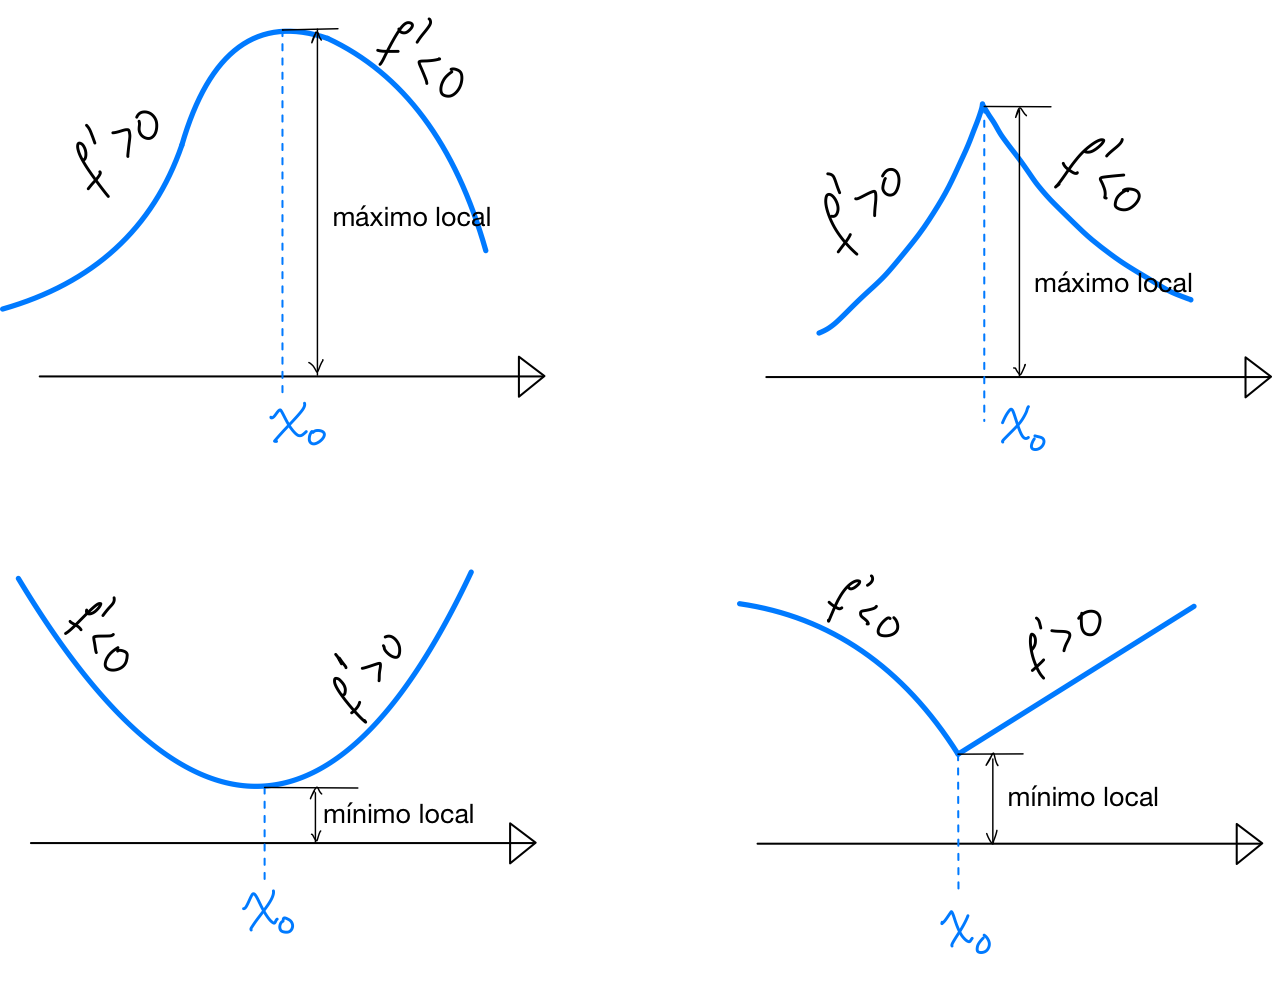
\includegraphics[width=.8\textwidth]{pics/max-min-locales-derivada.png}
}
La demostración es sencilla, haciendo uso de la Proposición~\ref{P:signo-derivada=>tendencia}.
\begin{proof}
    \begin{enumerate}
        \item Por la Proposición~\ref{P:signo-derivada=>tendencia}, $f$ es creciente en $[x_0-\delta,x_0]$ y decreciente en $[x_0,x_0+\delta]$, por lo tanto $f(x_0)\ge f(x)$, para todo $x\in[x_0-\delta,x_0+\delta]$.
        \item Por la Proposición~\ref{P:signo-derivada=>tendencia}, $f$ es decreciente en $[x_0-\delta,x_0]$ y creciente en $[x_0,x_0+\delta]$, por lo tanto $f(x_0)\le f(x)$, para todo $x\in[x_0-\delta,x_0+\delta]$.
        \item Hay aquí dos casos:
        \begin{enumerate}
            \item $f'(x)<0$ en $(x_0-\delta,x_0)$ y en $(x_0,x_0+\delta)$. En este caso, por la Proposición~\ref{P:signo-derivada=>tendencia}, $f$ es estrictamente decreciente en $[x_0-\delta,x_0+\delta]$.
            Por lo tanto, $f(x_0)<f(x)$, para todo $x\in (x_0-\delta,x_0)$; y
            $f(x_0)>f(x)$, para todo $x\in (x_0,x_0+\delta)$.
            \item $f'(x)>0$ en $(x_0-\delta,x_0)$ y en $(x_0,x_0+\delta)$. En este caso, por la Proposición~\ref{P:signo-derivada=>tendencia}, $f$ es estrictamente creciente en $[x_0-\delta,x_0+\delta]$.
            Por lo tanto, $f(x_0)>f(x)$, para todo $x\in (x_0-\delta,x_0)$; y
            $f(x_0)<f(x)$, para todo $x\in (x_0,x_0+\delta)$.
        \end{enumerate}
        En ambos casos, $f(x_0)$ no es ni un máximo ni un mínimo local de $f$.\qedhere
    \end{enumerate}
\end{proof}

\begin{example}
    Consideremos la función $f(x) = 2x^3-x^4$ en $\R$. Su derivada es
    $$ f'(x) = 6\,x^2-4\,x^3 = 2\, x^2\, (3-2x).$$
    La derivada se anula en $x=0$ y en $x=3/2$. Resumimos el signo de $f'$ en la siguiente tabla:

    \begin{center}
\def\arraystretch{1.5}
\begin{tabular}{|c|c|c|}
            \hline
            $x \in(-\infty,0)$ & $x\in(0, 3/2)$ & $x\in(3/2,+\infty)$ \\
            \hline
            $f'>0$& 
            $f'>0$ & 
            $f'<0$ \\
            \hline
            $f$ crece & 
            $f$ crece & 
            $f$ decrece \\
            \hline
        \end{tabular}
    \end{center}
    Luego, $f$ tiene un máximo local en $x=3/2$, pero no tiene ni un máximo ni un mínimo local en $x=0$.
\end{example}

\begin{proposition}[Criterio de la derivada segunda]
    Supongamos que $f'(x_0)=0$ y que existe $f''(x_0)$.
    \begin{itemize}
        \item Si $f''(x_0)>0$, entonces $f$ tiene un mínimo local en $x_0$.
        \item Si $f''(x_0)<0$, entonces $f$ tiene un máximo local en $x_0$.
    \end{itemize}
\end{proposition}

\begin{proof}
    Veamos el primer caso, el segundo queda como ejercicio para el lector.
    Supongamos que $f'(x_0)=0$ y $f''(x_0)>0$. Como $f''(x_0)$ es la derivada de $f'(x_0)$ resulta que existe un $\delta>0$ tal que, 
    $$ 
    \text{si}\quad x_0-\delta<x_1<x_0<x_2<x_0+\delta, 
    \quad\implies\quad 
    \frac{f'(x_1)- f'(x_0)}{x_1-x_0}>0,\ \text{y}\ 
    \frac{f'(x_2)- f'(x_0)}{x_2-x_0}>0,
    $$
    como $x_1<x_0<x_2$, $x_1-x_0<0$ y $x_2-x_0>0$, luego,
    $$ 
    \text{si}\quad x_0-\delta<x_1<x_0<x_2<x_0+\delta, 
    \qquad\text{entonces}\quad 
    f'(x_1)< f'(x_0) = 0 <f'(x_2).
    $$
    Es decir, 
    $$
    f'(x)<0\quad\text{para $x\in(x_0-\delta,x_0)$}
    \qquad\text{y}\qquad
    f'(x)>0\quad\text{para $x\in(x_0,x_0+\delta)$}.
    $$
    Por el criterio de la derivada primera, $f$ tiene un mínimo local en $x_0$.
\end{proof}

\begin{example}
    Consideramos $f(x)=2\, x^3-3\, x^2-12\, x+5$, para la cual
    $$ f'(x) = 6\, x^2 - 6\, x-12 = 6(x^2-x-2) = 6(x-2)(x+1),
    $$ 
    y $$ f''(x) = 12\, x-6.$$
    Los puntos críticos son $x=2$ y $x=-1$; la derivada primera en cada uno de estos puntos es $0$.
    Dado que $f''(2)=18>0$ y $f''(-1)=-18<0$, podemos concluir por el criterio de la segunda $f(2)=-15$ es un mínimo local y $f(-1)=12$ es un máximo local.
\end{example}

\begin{example}
    Para mostrar lo que puede suceder si la derivada segunda es cero en un punto crítico $x_0$, consideremos las siguientes tres funciones:
    $$ f(x)=x^3,\qquad g(x)=x^4,\qquad, h(x)=-x^4. $$
    En cada caso, $x=0$ es un punto crítico, ya que
    $$ f'(x)=3\, x^2,\qquad g(x)=4\, x^3,\qquad, h(x)=-4 \, x^3; $$
    y también la derivada segunda de estas tres funciones se anula en $x=0$:
    $$ f''(x)=6\, x,\qquad g(x)=12\, x^2,\qquad, h(x)=-12 \, x^2. $$
    En el primer caso, $f(x)=x^3$ no tiene ni un máximo ni un mínimo local en $x=0$. En cambio $g(x)=x^4$ tiene un mínimo local y $h(x)=-x^4$ tiene un máximo local, lo que puede verificarse por el criterio de la derivada primera.
    
\end{example}


\subsubsection*{Ejercicios de la sección~\getcurrentref{chapter}.\getcurrentref{section}}

\begin{enumerate}

\item Hallar el mínimo de la función $f:(0,+\infty)\to \R$ dada por $\D f(x) = x + \frac1x$.

\item Hallar las dimensiones del cilindro circular recto de volumen $V$ que tenga mínima área exterior. (Si el cilindro tiene base circular de radio $r$ y altura $h$, entonces el volumen es: $\pi \, r^2\, h$ y el área exterior es $2\pi \, r^2 + 2 \pi \, r\, h$).

\item Consideremos la función $(x-1)^2+(x-3)^2+(x-5)^2$. Graficarla en Geogebra, y encontrar el valor mínimo y el punto mínimo.

\item Dados $a_1<a_2<\dots <a_n$, hallar el valor de $x$ que minimiza $\sum_{i=1}^n (a_i-x)^2$.

\item La siguientes figuras muestran la gráfica de \emph{la derivada $f'$ de $f$}. Hallar:
\begin{itemize}
  \item Todos los puntos máximos y mínimos locales de $f$.
  \item Intervalos de crecimiento y decrecimiento de $f$.
  \item Intervalos de convexidad y concavidad de $f$, y puntos de inflexión.
\end{itemize} 

\begin{multicols}{2}
  \begin{enumerate}
    \item 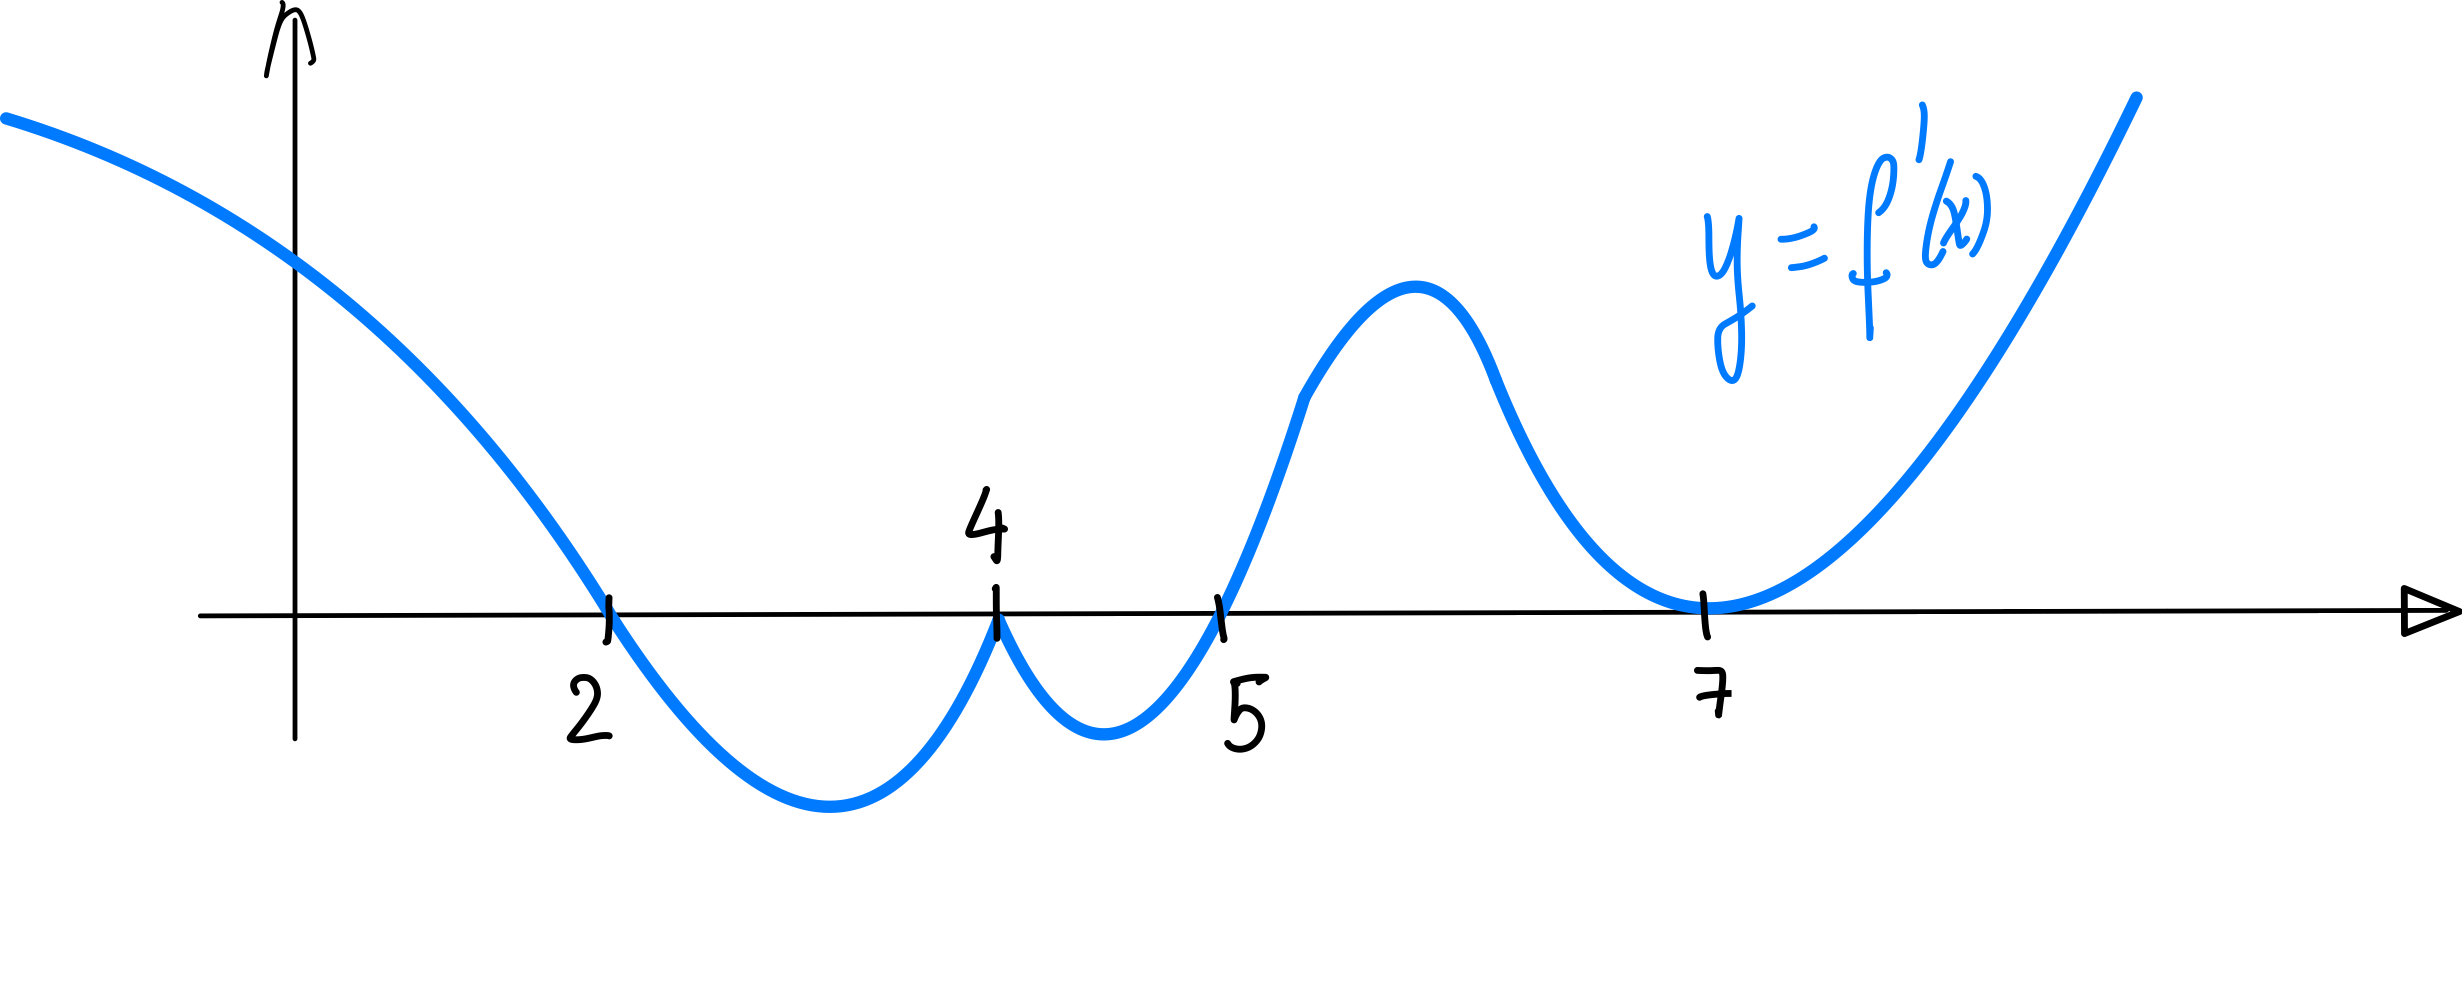
\includegraphics[width=.4\textwidth]{pics/max-min-locales-ej-a.png}
    \item 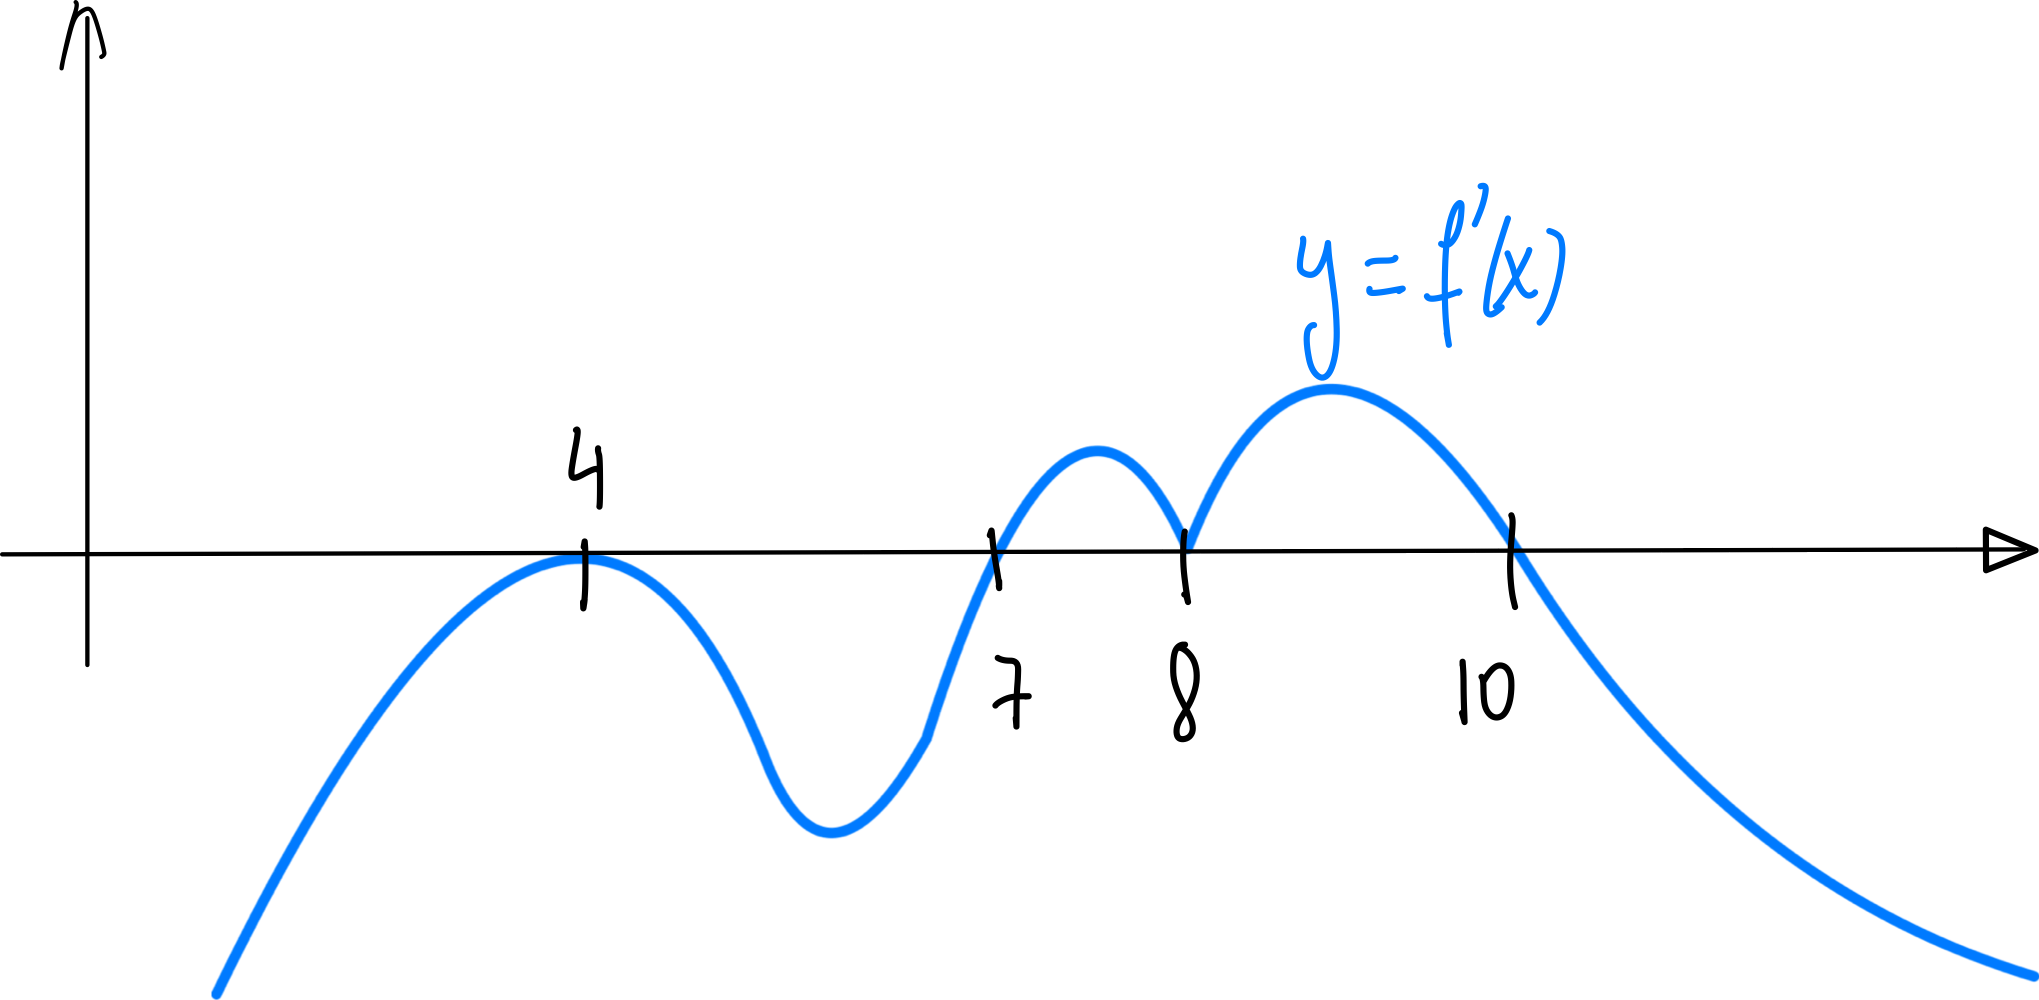
\includegraphics[width=.4\textwidth]{pics/max-min-locales-ej-b.png}
    \item 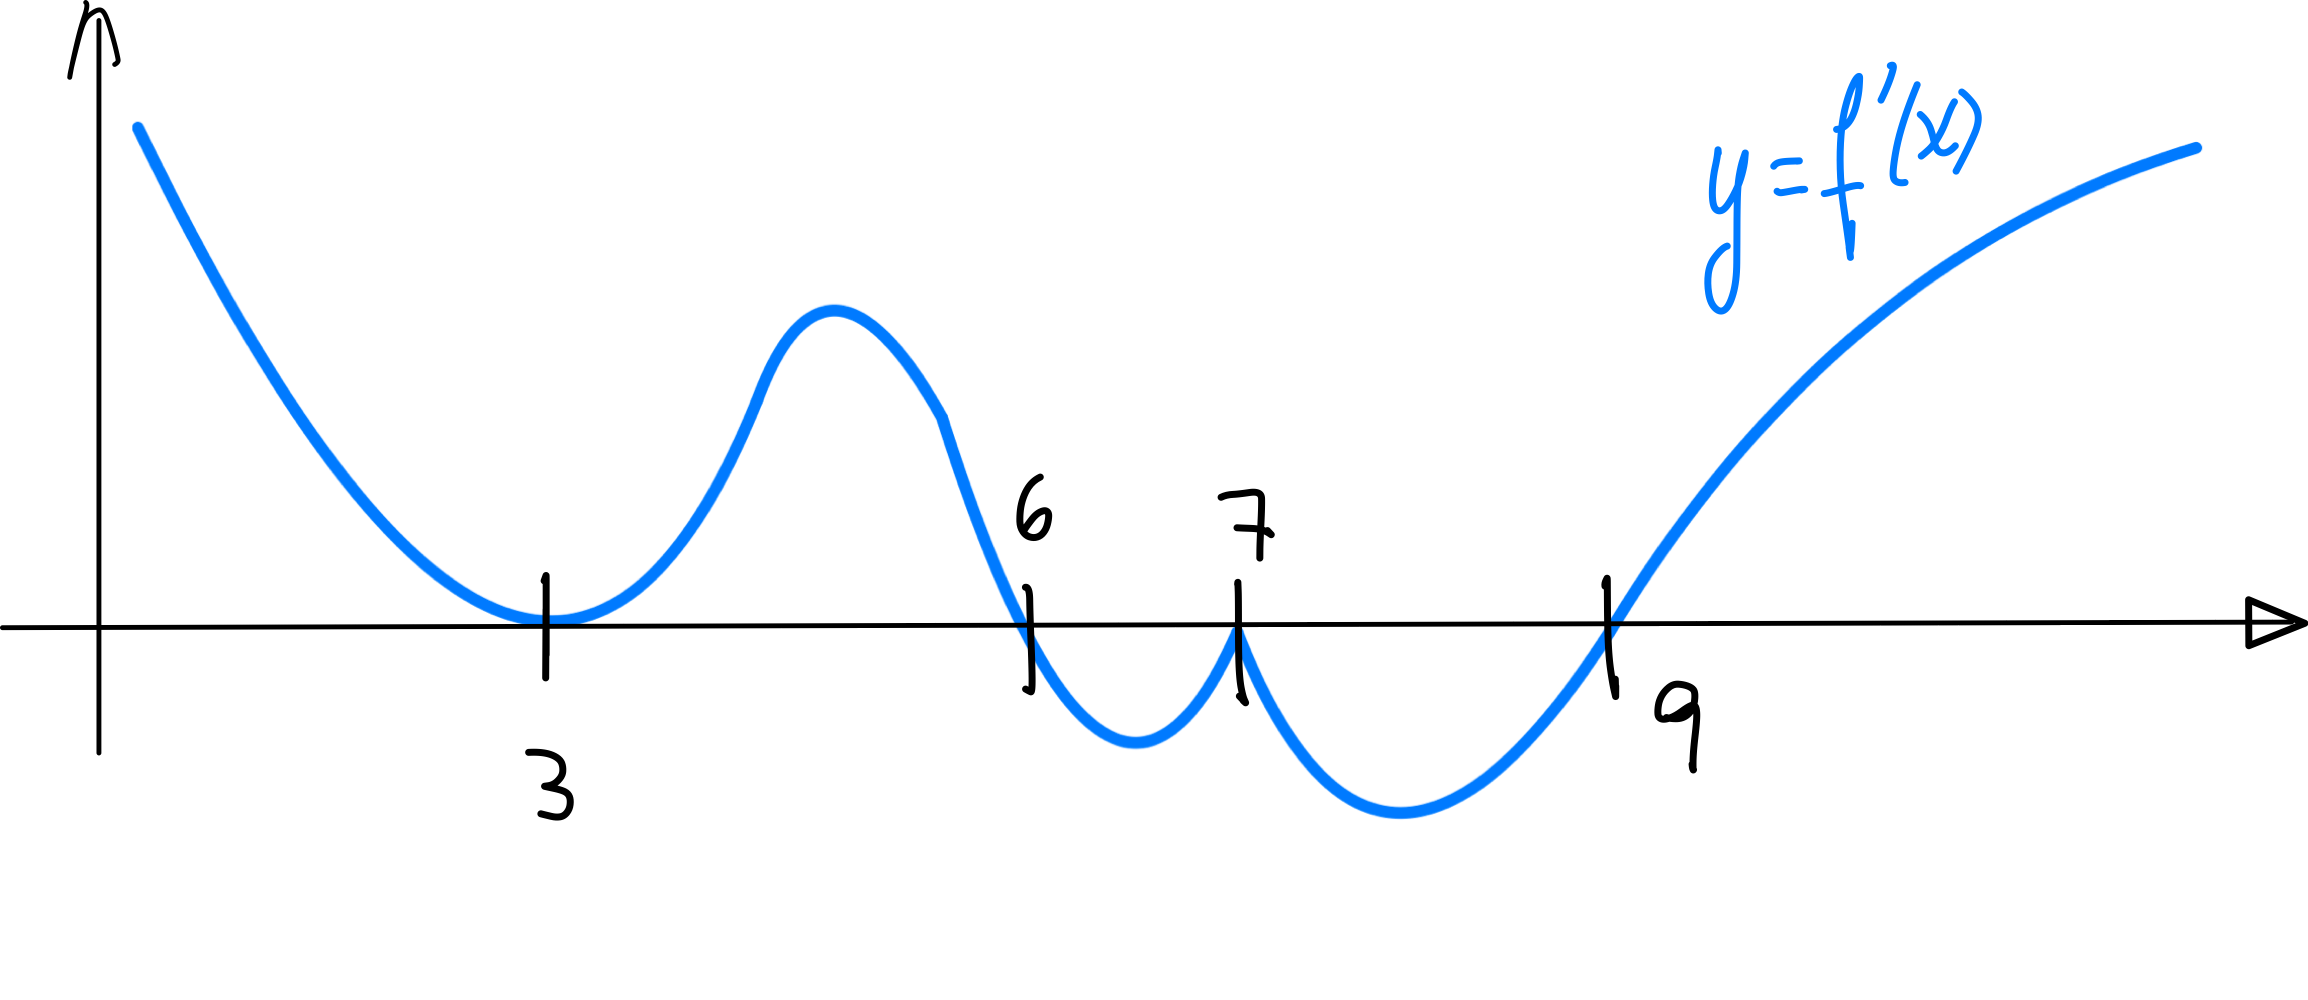
\includegraphics[width=.4\textwidth]{pics/max-min-locales-ej-c.png}
    \item 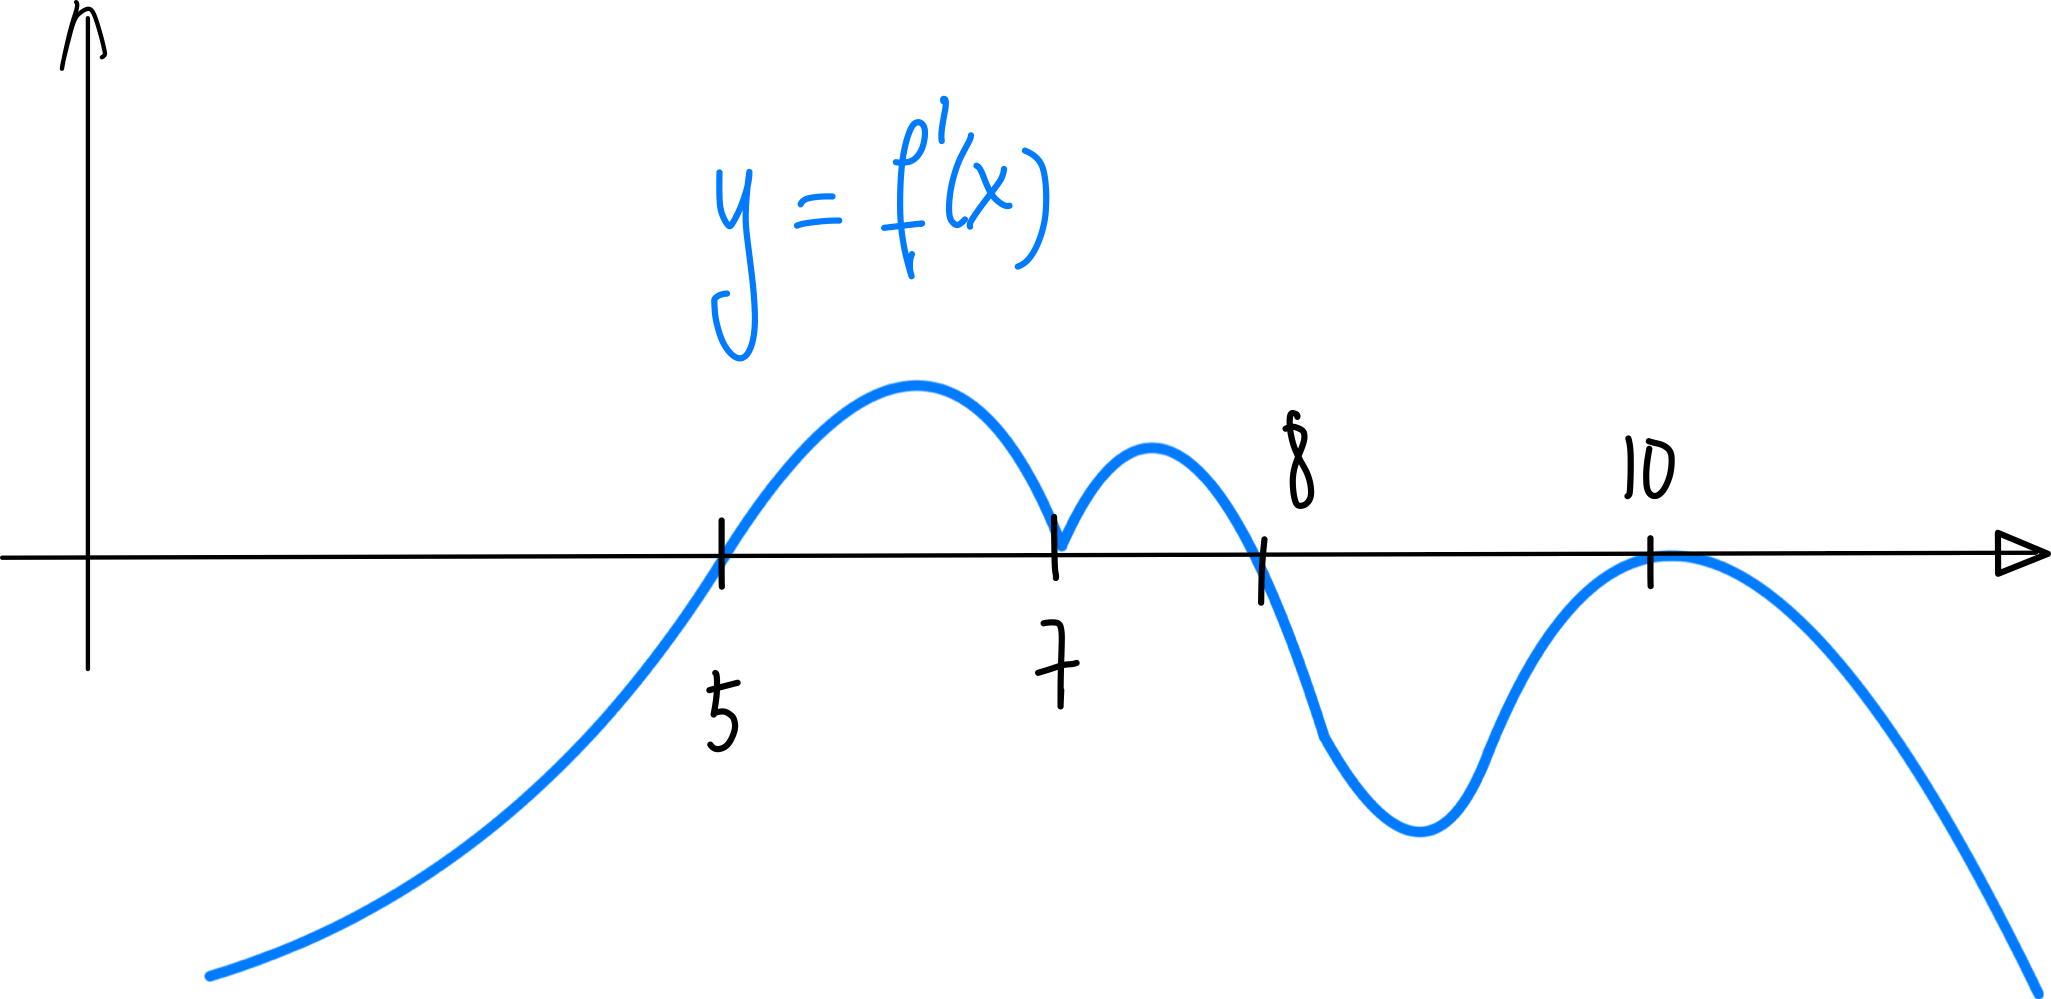
\includegraphics[width=.4\textwidth]{pics/max-min-locales-ej-d.png}
  \end{enumerate}
  
\end{multicols}

\end{enumerate}


\section{Regla de L'Hospital}

\begin{comment}
Vemos ahora un Teorema del Valor Medio Generalizado:
\begin{theorem}[Teorema del Valor Medio Generalizado (de Cauchy)]
    Si $f$ y $g$ son continuas en $[a,b]$ y derivables en $(a,b)$, entonces existe $c\in(a,b)$ tal que
    \[
        \big( f(b)-f(a) \big) \cdot g'(c) = \big( g(b)-g(a) \big)\cdot f'(c).
    \]
    Si, además $g'(x)\neq 0$ para todo $x\in(a,b)$, entonces
    \[
    \frac{f(b)-f(a)}{g(b)-g(a)}=\frac{f'(c)}{g'(c)}.
    \]
\end{theorem}

\begin{proof}
    Consideremos la función
    \[
    h(x) = \big( f(b)-f(a) \big) \cdot \big(g(x)-g(a)\big) 
    - \big( g(b)-g(a) \big)\cdot \big(f(x)-f(a)\big).
    \]
    Esta función $h(x)$ es continua en $[a,b]$ y derivable en $(a,b)$ por ser producto y suma de funciones de ese tipo. Además:
    \begin{align*}
        h(a) &= \big( f(b)-f(a) \big) \cdot \big(g(a)-g(a)\big) 
        - \big( g(b)-g(a) \big)\cdot \big(f(a)-f(a)\big) = 0,
        \\
        h(b) &= \big( f(b)-f(a) \big) \cdot \big(g(b)-g(a)\big) 
        - \big( g(b)-g(a) \big)\cdot \big(f(b)-f(a)\big) = 0.
    \end{align*}
    Entonces $h$ satisface las hipótesis del Teorema de Rolle, y existe $c\in(a,b)$ tal que $h'(c)=0$. Pero
    \[
        h'(x) = \big( f(b)-f(a) \big) \cdot g'(x)
        - \big( g(b)-g(a) \big)\cdot f'(x).
    \]
    Luego, $\D \big( f(b)-f(a) \big) \cdot g'(c)
    - \big( g(b)-g(a) \big)\cdot f'(c)= 0$, que es lo que se quería demostrar.
\end{proof}

Como consecuencia de este teorema, vemos un resultado que nos da una igualdad de mucha utilidad para el cálculo de límites.


\begin{proposition}[Regla de L'Hospital, caso $0/0$]
    Sean $f$ y $g$ funciones definidas y derivables en un intervalo $(a,b)$.
    Para $x_0\in(a,b)$, supongamos que $g'(x)\neq 0$, para todo $x\neq x_0$ y $f(x_0)=g(x_0)=0$.
    Bajo estas hipótesis, si existe $\D\limxo \frac{f'(x)}{g'(x)}=\ell$, entonces existe $\D\limxo \frac{f(x)}{g(x)}$ y además $\D\limxo \frac{f(x)}{g(x)}=\ell$, es decir
    \[
        \limxo \frac{f(x)}{g(x)}=\limxo \frac{f'(x)}{g'(x)}.
    \]
\end{proposition}

\begin{proof}
    Sea $\ell = \limxo \frac{f'(x)}{g'(x)}=\ell$. Entonces, dado $\epsilon>0$, existe $\delta>0$ tal que
    \[
    0<|x-x_0|<\delta\quad\implies\quad \Big| \frac{f'(x)}{g'(x)}-\ell \Big|<\epsilon.\]
    Ahora bien, para cada $x$ tal que $0<|x-x_0|<\delta$, existe $c$ entre $x$ y $x_0$, tal que
    \[
    \frac{f(x)}{g(x)}=\frac{f(x)-f(x_0)}{g(x)-g(x_0)} = \frac{f'(c)}{g'(c)}.
    \]
    Como $c$ está entre $x$ y $x_0$, resulta que $0<|c-x_0|<|x-x_0|<\delta$, y entonces
    \[
    \Big| \frac{f(x)}{g(x)}-\ell\Big| 
    = 
    \Big| \frac{f'(c)}{g'(c)}-\ell\Big| < \epsilon.
    \]
    Hemos demostrado entonces que, dado $\epsilon>0$, existe $\delta>0$ tal que
    \[
        \Big| \frac{f(x)}{g(x)}-\ell\Big| <\epsilon,
        \quad\text{para todo $x$ tal que $0<|x-x_0|<\delta$}.
    \]    
    Es decir, $\D\limxo \frac{f(x)}{g(x)}=\ell$.
\end{proof}

\end{comment}

El siguiente teorema nos da una igualdad de mucha utilidad para el cálculo de límites:

\begin{proposition}[Regla de L'Hospital, caso $0/0$]
    Sean $f$ y $g$ funciones definidas y derivables en un intervalo $(a,b)$.
    Supongamos que para $x_0\in(a,b)$ queremos calcular $\D\limxo \frac{f(x)}{g(x)}$, pero $f(x_0)=\limxo f(x)=0$ y $g(x_0)=\limxo g(x)=0$, es decir, tenemos un indeterminado del tipo $\frac00$.
    Supongamos también que $f'$ y $g'$ son continuas en $(a,b)$.
    Si $g'(x_0)\neq 0$, entonces existe $\D\limxo \frac{f(x)}{g(x)}$ y además $\D\limxo \frac{f(x)}{g(x)}=\frac{f'(x_0)}{g'(x_0)}$, es decir
    \[
        \limxo \frac{f(x)}{g(x)}=\frac{f'(x_0)}{g'(x_0)}=\limxo \frac{f'(x)}{g'(x)}.
    \]
\end{proposition}

\begin{proof}
    Recordemos primero que $\D\limxo \frac{f(x)}{g(x)}=\limho \frac{f(x_0+h)}{g(x_0+h)}$. Y por la definición alternativa de derivada~\eqref{eq:derivada-o(h)}
    \begin{align*}
        f(x_0+h) &= \underbrace{f(x_0)}_{0} + h \cdot f'(x_0) + o(h) = h \cdot f'(x_0) + o(h),\\
        g(x_0+h) &= \underbrace{g(x_0)}_{0} + h \cdot g'(x_0) + o(h) = h \cdot g'(x_0) + o(h).
    \end{align*}
    Luego
    \begin{align*}
        \frac{f(x_0+h)}{g(x_0+h)} &= \frac{ h \cdot f'(x_0) + o(h)}{h \cdot g'(x_0) + o(h)}
        = \frac hh  \cdot \frac{ f'(x_0) + \frac{o(h)}h}{ g'(x_0) + \frac{o(h)}h}
        \toh{0} \frac{f'(x_0) + 0}{g'(x_0) + 0}
        = \frac{  f'(x_0)}{ g'(x_0)}.
    \end{align*}
    Es decir, $\D\limxo \frac{f(x)}{g(x)}=\frac{f'(x_0)}{g'(x_0)}=\limxo \frac{f'(x)}{g'(x)}$.
\end{proof}
    
\begin{example}
    Utilizaremos esta regla para calcular $\D\lim_{x\to 1} \frac{\ln x}{x-1}$.
    El numerador y el denominador tienden a $0$ cuando $x\to1$:
    \[
        \lim_{x\to 1} \ln x = \ln 1 = 0,
        \qquad
        \lim_{x\to 1} (x-1) = 1-1=0.
    \]
    Por lo tanto es un límite indeterminado de la forma $\frac00$. Si derivamos el numerador y el denominador tenemos
    \[
    \frac{d \ln x}{dx} = \frac1x\tox{1}1, \qquad \frac{d(x-1)}{dx}=1\tox{1}1.
    \]
    Calculamos ahora el límite del cociente de estas dos derivadas:
    \[
        \lim_{x\to 1} \frac{\ln x}{x-1}= \lim_{x\to 1} \frac{\frac{d \ln x}{dx}}{\frac{d(x-1)}{dx}}
    =\lim_{x\to 1} \frac{\frac1x}{1}=\lim_{x\to 1} \frac1x=1.
    \]
\end{example}

\begin{example}
    La regla de L'Hospital puede aplicarse de manera repetida. Por ejemplo, para calcular $\D\lim_{x\to 0}\frac{1-\cos x}{x^2}$ que otra vez es del tipo $\frac00$, observamos que 
    \[
    \dd[]{(1-\cos x)}{x}=0-(-\sen x)=\sen x,
    \quad\text{y}\quad
    \dd[]{x^2}{x}=2x.
    \]
    Ambas derivadas tienden a cero cuando $x\to 0$, por lo tanto seguimos teniendo un \emph{indeterminado}. Volvemos a derivar
    \[
        \dd[]{\sen x}{x}=\cos x,
        \quad\text{y}\quad
        \dd[]{2x}{x}=2.
    \]
    Estas nuevas derivadas tienden a $1$ y a $2$, respectivamente, cuando $x\to 0$, por lo tanto, $\D\lim_{x\to 0}\frac{1-\cos x}{x^2}=\frac12$. Todo este razonamiento es muy complicado de escribir de esta manera.
    
    Una manera más sencilla de escribirla es la siguiente:
    \[
        \lim_{x\to 0}\frac{1-\cos x}{x^2}
        \eqLH \lim_{x\to 0}\frac{\sen x}{2x}
        \eqLH \lim_{x\to 0}\frac{\cos x}{2} = \frac12.
    \]
    Donde usamos \,$\eqLH$\, para indicar que en ese paso estamos usando la regla de L'Hospital.
\end{example}


\begin{proposition}[Regla de L'Hospital, caso $\infty/\infty$]
    Sean $f$ y $g$ funciones definidas y derivables en un intervalo $(a,b)$.
    Para $x_0\in(a,b)$, supongamos que $\limxo f(x)=\limxo g(x)=\infty$.
    Bajo estas hipótesis, si existe $\D\limxo \frac{f'(x)}{g'(x)}=\ell$, entonces existe $\D\limxo \frac{f(x)}{g(x)}$ y además $\D\limxo \frac{f(x)}{g(x)}=\ell$, es decir
    \[
        \limxo \frac{f(x)}{g(x)}=\limxo \frac{f'(x)}{g'(x)}.
    \]
\end{proposition}

La demostración de esta proposición y las que siguen a continuación quedan fuera del alcance de este apunte, y serán discutidas en los \emph{Coloquios de Demostraciones}.

\begin{proposition}[Regla de L'Hospital, 2$^{\text{do}}$ caso $0/0$]
    Sean $f$ y $g$ funciones definidas y derivables en un intervalo $(a,b)$.
    Para $x_0\in(a,b)$, supongamos que $g'(x)\neq 0$, para todo $x\neq x_0$ y $f(x_0)=g(x_0)=0$.
    Bajo estas hipótesis,
    \[
    \text{si}\quad \D\limxo \frac{f'(x)}{g'(x)}=\infty
    \quad\text{entonces}\quad
    \D\limxo \frac{f(x)}{g(x)}=\infty.
    \]
\end{proposition}

\begin{proposition}[Regla de L'Hospital, 2$^{\text{do}}$ caso $\infty/\infty$]
    Sean $f$ y $g$ funciones definidas y derivables en un intervalo $(a,b)$.
    Para $x_0\in(a,b)$, supongamos que $\limxo f(x)=\limxo g(x)=\infty$.
    Bajo estas hipótesis, 
    \[
    \text{si}\quad \D\limxo \frac{f'(x)}{g'(x)}=\infty
    \quad\text{entonces}\quad
    \D\limxo \frac{f(x)}{g(x)}=\infty.
    \]
\end{proposition}



\subsubsection*{Ejercicios de la sección~\getcurrentref{chapter}.\getcurrentref{section}}

\begin{enumerate}
\item Calcular los siguientes límites:
\begin{multicols}{2}
  \begin{enumerate}
    \item $\D \lim_{x\to 0} \frac{x-\sen x}{x^3}$
    \item $\D \lim_{x\to 2} \frac{x^2-4}{x-2}$
    \item $\D \lim_{x\to a} \frac{x^2-a^2}{x-a} $
    \item $\D \lim_{x\to 0} \frac{\sen (5x)}x$
    \item $\D \lim_{x\to 1} \frac{x^2-2x+1}{3x^2+2x-5} $
    \item $\D \lim_{x\to 0} \frac{e^{2x}-e^{-2x}-4x}{x-\sen x}$
    \item $\D \lim_{x\to a} \frac{x^n-a^n}{x-a}$
    \item $\D \lim_{x\to 0} \frac{\tan x-x}{x-\sen x}$
    \item $\D \lim_{x\to \frac\pi2} \frac{\ln(\sen x)}{\pi -2x}$
    \item $\D \lim_{x\to a} \frac{\sen x - \sen a}{x-a}$
    \item $\D \lim_{x\to 0} \frac{(a+x)^x-a^x}{x^2}$ ($a>0$)
    \item $\D \lim_{x\to +\infty} \frac{\ln x}{x^2}$
    \item $\D \lim_{x\to +\infty} \frac{\ln x}{x^{0.1}}$
    \item $\D \lim_{x\to +\infty} \frac{e^x}{x^n}$ (\niN)
    \item $\D \lim_{x\to +\infty} \frac{e^x}{\sqrt{x}}$
    \item $\D \lim_{x\to +\infty} \frac{x+\ln x}{x\, \ln x}$
    \item $\D \lim_{x\to +\infty} \frac{\ln x}{e^x}$
    \item $\D \lim_{x\to +\infty} \frac{\sen (1/x)}{1/x}$
    \item $\D \lim_{x\to 0^+} x^2 \, \ln x$
    \item $\D \lim_{x\to 0^+} (x-\sen x) \, \ln x$
    \item $\D \lim_{x\to 0} \big( \frac1x-\frac{\cos x}{\sen x}\big)$
  \end{enumerate}
\end{multicols}

\item Para calcular $\D\limxo f(x)^{g(x)}$ en los casos de indeterminación ($1^\infty$, $0^0$, $\infty^0$) suele ser útil calcular el logaritmo del límite:
\[
\ln \big(\limxo f(x)^{g(x)}\big) = \limxo \ln \big(f(x)^{g(x)}\big)
= \limxo \big[ g(x) \, \ln f(x) \big] = \limxo \frac{\ln f(x)}{1/g(x)}.
\]
Para aplicar este último límite puede ser útil aplicar L'Hospital. Si se encuentra el límite $\ell$, luego el límite original será $e^\ell$.

Aplicar este procedimiento apra calcular los siguientes límites:
\begin{multicols}{2}
  \begin{enumerate}
    \item $\D \lim_{x\to 0}x^{\sen x}$
    \item $\D \lim_{x\to +\infty}\big(1+\frac ax)^x$
    \item $\D \lim_{x\to +\infty}(1+x)^{1/x}$
    \item $\D \lim_{x\to 0^+} (-\ln x)^x$
    \item $\D \lim_{x\to 0^+} \Big(\frac{\tan x}x\Big)^{1/x^2} $
    \item $\D \lim_{x\to \pi/2} (\sen x)^{\tan x}$
    \item $\D \lim_{x\to +\infty} \Big(\frac{\ln x}{x}\Big)^{1/x}$
    \item $\D \lim_{x\to 0} x^x$
    \item $\D \lim_{x\to 0} x^{x^x}$
  \end{enumerate}
\end{multicols}

\item Calcular primero los límites siguientes sin utilizar L'Hospital.
?`Qué ocurre si se intenta aplicar L'Hospital?
\begin{multicols}{2}
  \begin{enumerate}
    \item $\D \lim_{x\to 0}\frac{x^2\,\sen(1/x)}{\sen x}$
    \item $\D \lim_{x\to +\infty}\frac{x+\sen x}{x+\cos x}$
  \end{enumerate}
\end{multicols}
Volver a interpretar el Teorema de L'Hospital en vistas de estas observaciones.


\end{enumerate}


\section{Estudio de funciones}


\subsubsection*{Ejercicios de la sección~\getcurrentref{chapter}.\getcurrentref{section}}

\begin{enumerate}
\item 
\end{enumerate}



\subsection*{Ejercicios del capítulo~\getcurrentref{chapter}}



